\chapter{CNNs in Depth}


\section{Why Should I Learn to Build a CNN from Scratch?}
In this lesson we are going to learn how to build and train a CNN from scratch.

However, in real-world situation, it is far more common to fine-tune an existing architecture than to build one from scratch.

Does this mean that this lesson is not needed? Of course not!

Understanding how things work in some detail is going to be very useful (and fun!). It will allow you to understand the strength and the limitations of different methods and architectures, as well as to follow and understand the state-of-the-art which evolves quickly.

Also, in some situations a slight modification to an existing architecture can make all the difference. You won't know where to start if you don't know at least at a high-level how things work internally.

So every expert would agree that starting from fundamentals and building your way up is the way to go. So let’s get started!

\section{Convolutional Layers in Depth}

\subsection{Convolution}

You have learned about the concept of convolution as applied to grayscale images. \newline

You now also understand how convolution can extract features such as edges that can be used to recognize what the image represents. \newline

Let's recap some of these concepts and go deeper, extending convolutions to color images. \newline

\href{https://www.youtube.com/watch?v=Cq7rqxi_x3I&t=2s&ab_channel=Udacity}{Youtube} \newline

\subsection{Greyscale images}
Recall the case of a single convolutional filter. Adding another filter is probably exactly what you'd expect where we just populate an additional collection of nodes in the convolutional layer. This collection has its own shared set of weights that differ from the weights for the blue nodes above them.

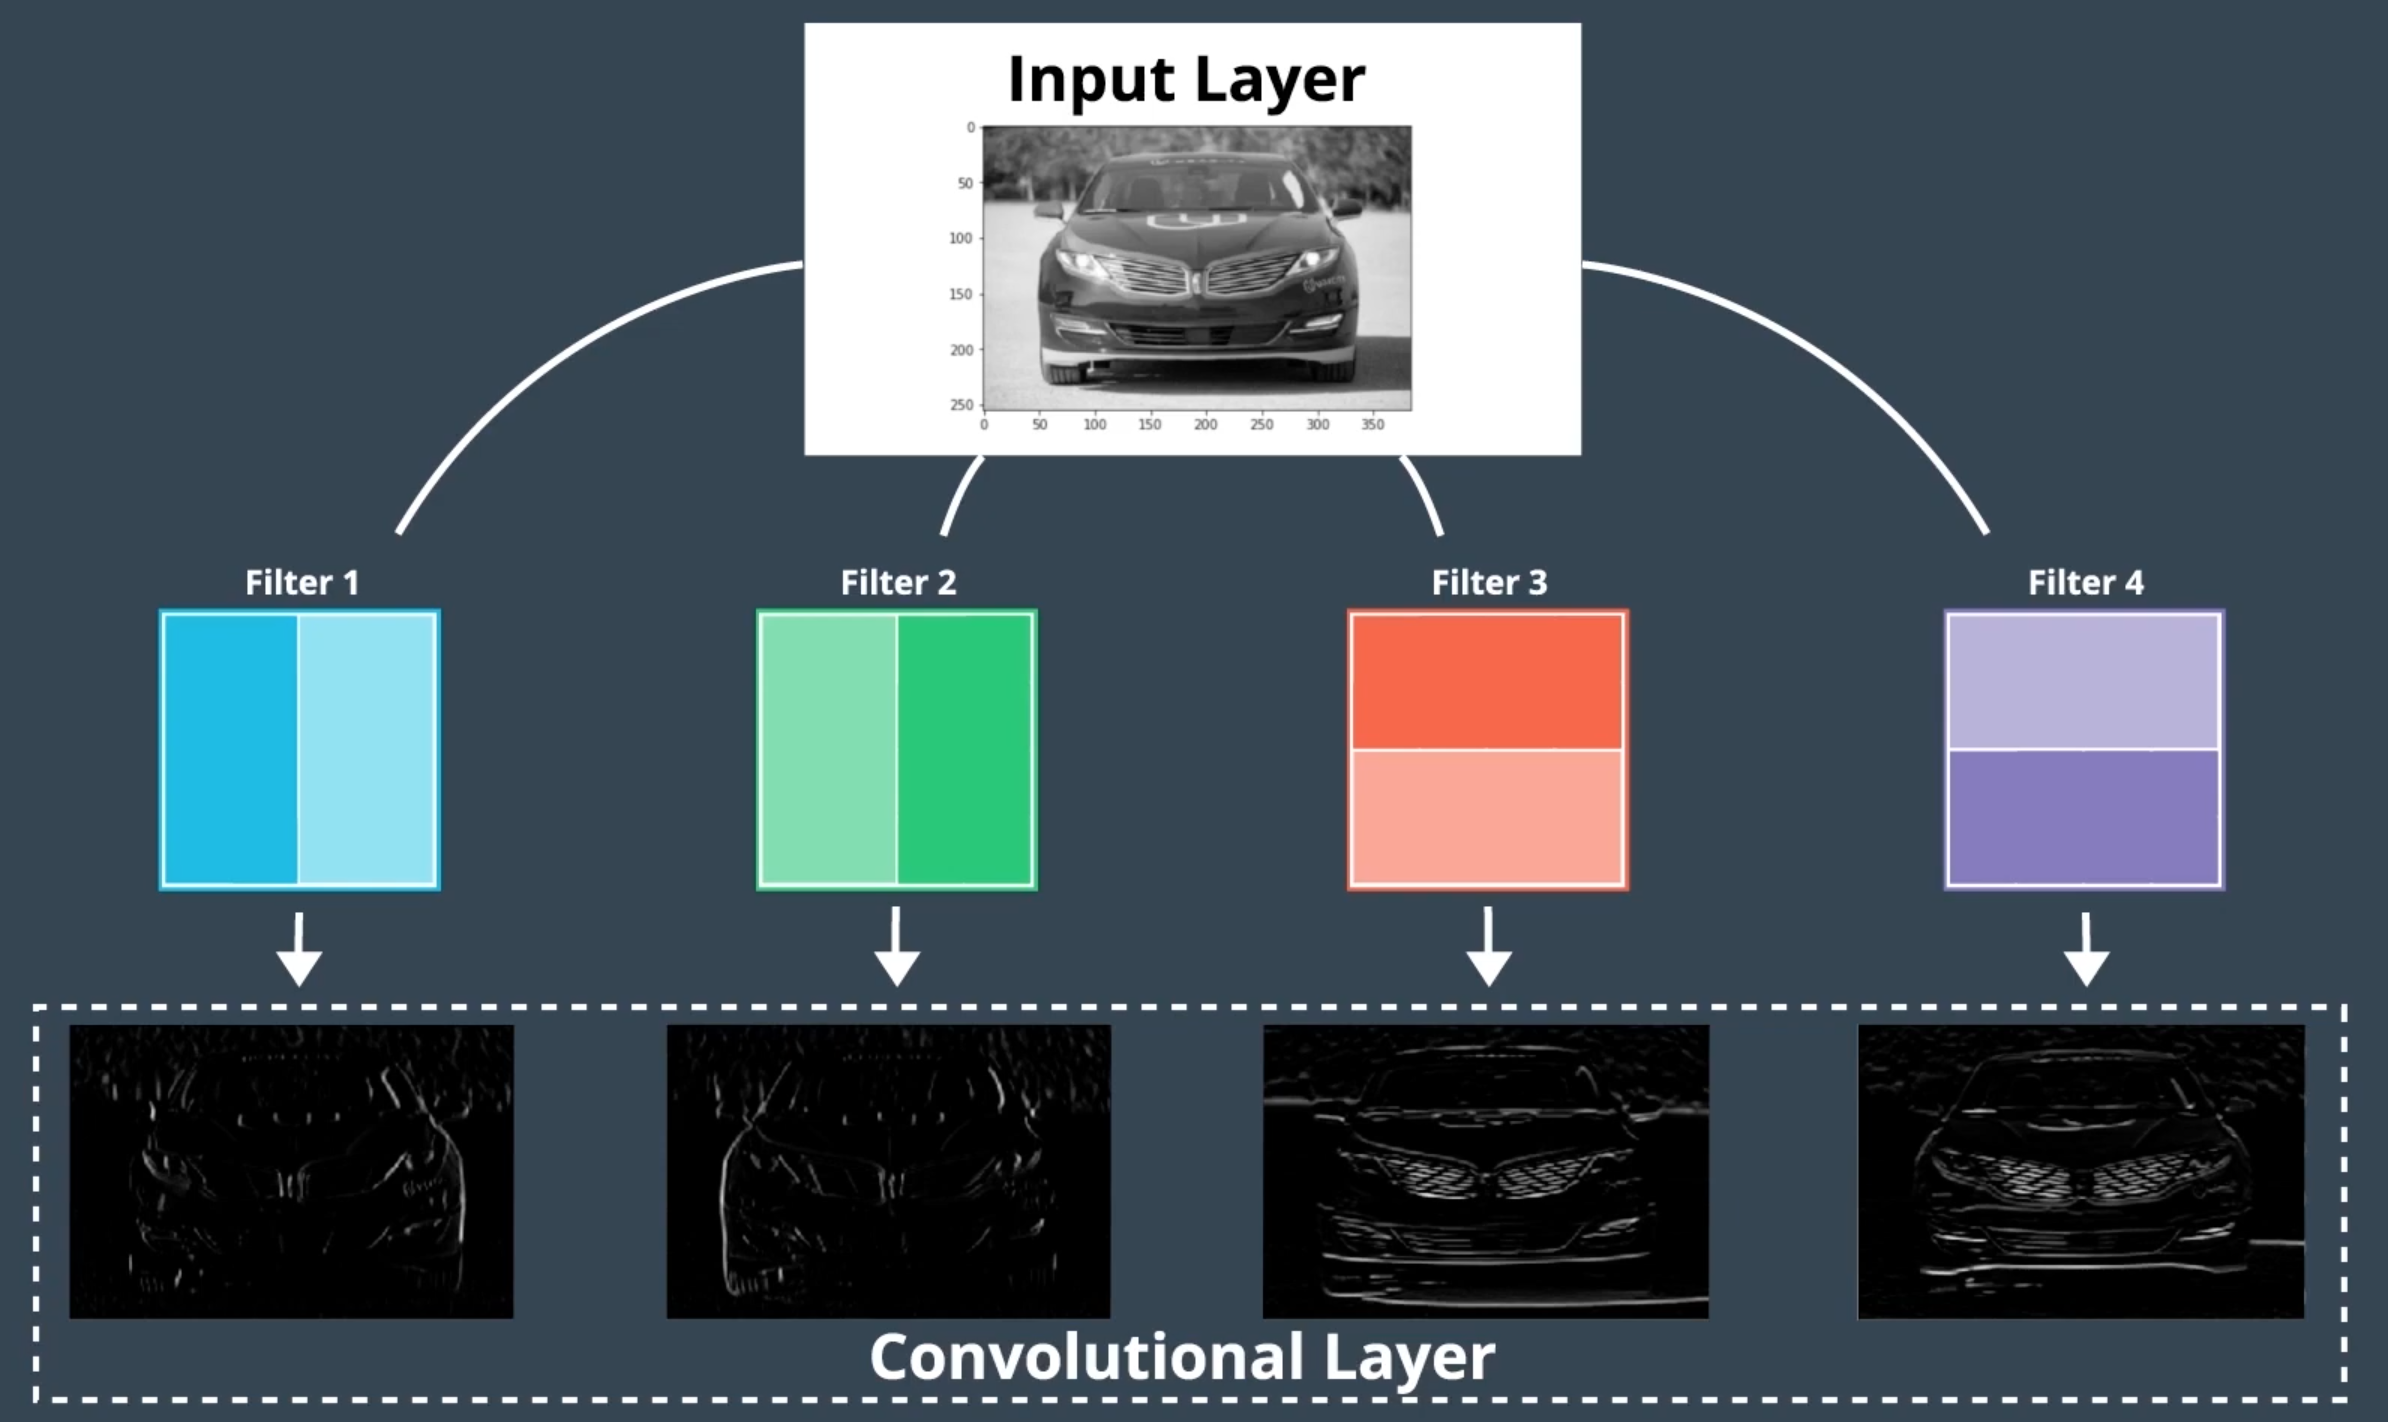
\includegraphics[width=0.75\linewidth]{img//cnn//depth/image2.png}
\captionof{figure}{ }
\label{fig:cnnUberCar}

Say we're working with an image of Udacity's self-driving car as input.
We use four filters each four pixels high and four pixels wide. Each filter will be convolved across the height and width of the image to produce an entire collection of nodes in the convolutional layer. Since we have four filters, we have four collections of nodes. In practice, we refer to each of these four collections as either feature maps or as activation maps. When we visualize these feature maps, we see that they look like filtered images. That is, we've taken all of the complicated, dense information in the original image and in each of these four cases, outputted a much simpler image with less information (see \autoref{fig:cnnUberCar}).
The first two filters discover vertical edges while the last two detect horizontal edges in the image.
Remember that lighter values in a feature map mean that the pattern in the filter was detected in the image. \newline

Can you match the lighter regions in each feature map with their corresponding areas in the original image? In the second activation map, we can see a clear white line to finding the right edge of the car. This is because all of the corresponding regions in the car image closely resemble
the filter where we have a vertical line of dark pixels to the left of a vertical line of lighter pixels.
If you think about it, you'll notice that edges in images appear as a line of lighter pixels next to a line of darker pixels. \newline

Grayscale images are interpreted by the computer as a 2D array with height and width. Color images are interpreted by the computer as a 3D array with height, width, and depth. In the case of RGB images, the depth is three. This 3D array is best conceptualized as a stack of three, 2-dimensional matrices, where we have matrices corresponding to the red, green, and blue channels of the image.

\subsection{Convolution on Color Images}

In this video we have shown how to apply convolution to color images. The kernel that was a matrix of k x k numbers for grayscale images, becomes now a 3d filter of k x k x n channels:

% \includegraphics[width=0.5\linewidth]{img//cnn//depth/main-qimg-b662a8fc3be57f76c708c171fcf29960.gif}
\captionof{figure}{Convolution on Color Images}


\subsection{Multiple Convolutional Layers}

In a CNN with more than one layer, the nk filters in the first convolutional layer will operate on the input image with 1 or 3 channels (RGB) and generate nk output feature maps. So in the case of an RGB image the filters in the first convolutional layer will have a shape of kernel\_size x kernel\_size x 3. If we have 64 filters we will then have 64 output feature maps. Then, the second convolutional layer will operate on an input with 64 "channels" and therefore use filters that will be kernel\_size x kernel\_size x 64. Suppose we use 128 filters. Then the output of the second convolutional layer will have a depth of 128, so the filters of the third convolutional layer will be kernel\_size x kernel\_size x 128, and so on. For this reason, it is common to use the term "channels" also to indicate the feature maps of convolutional layers: a convolutional layer that takes feature maps with a depth of 64 and outputs 128 feature maps is said to have 64 channels as input and 128 as outputs.

\subsection{Number of Parameters in a Convolutional Layer}

Let's see how we can compute the number of parameters in a convolutional layer,  \(n_p\). \newline

Let's define some quantities:
\begin{itemize}
    \item \(n_k\): number of filters in the convolutional layer
    \item k: height and width of the convolutional kernel
    \item c: number of feature maps produced by the previous layer (or number of channels in input image)
\end{itemize}

There are k times k times c weights per filter plus one bias per filter, so \(c \cdot k^2 + 1\) parameters. The convolutional layer is composed of \(n_k\) filters, so the total number of parameters in the convolutional layer is:
\[n_p = n_k (c \cdot k^2 + 1)\]
\captionof{figure}{Formula to compute number of parameters in convolutional layer}


\section{Convolutional Layers in PyTorch}

\subsection{Convolutional Layers in PyTorch}

To create a convolutional layer in PyTorch, you must first import the necessary module:
\begin{lstlisting}
from torch import nn
\end{lstlisting}

Then you can define a convolutional layer as:
\begin{lstlisting}
conv1 = nn.Conv2d(in_channels, out_channels, kernel_size)
\end{lstlisting}
You must pass the following arguments:

\begin{itemize}
    \item \lstinline{in_channels} - The number of input feature maps (also called channels). If this is the first layer, this is equivalent to the number of channels in the input image, i.e., 1 for grayscale images, or 3 for color images (RGB). Otherwise, it is equal to the output channels of the previous convolutional layer.
    \item \lstinline{out_channels} - The number of output feature maps (channels), i.e. the number of filtered "images" that will be produced by the layer. This corresponds to the unique convolutional kernels that will be applied to an input, because each kernel produces one feature map/channel. Determining this number is an important decision to make when designing CNNs, just like deciding on the number of neurons is an important decision for an MLP.
    \item \lstinline{kernel_size} - Number specifying both the height and width of the (square) convolutional kernel.
\end{itemize}
There are also some additional, optional but important arguments that we are going to see in the next video. \newline

At any time consult the official PyTorch \href{https://pytorch.org/docs/stable/generated/torch.nn.Conv2d.html\#torch.nn.Conv2d}{\textbf{documentation}} for more details and further options. \newline

Note in PyTorch that this convolutional layer does NOT include the activation function, which is different than in other deep learning libraries such as Keras. We need to add that as a separate layer.

\subsection{Adding the Activation Function and Dropout}

As we have seen in the case of MLPs, the activation function must be specified as a separate layer. The same is true for the Dropout layer, which is a very effective regularizer for neural networks. In the case of CNNs, we need to use the 2d version of Dropout, which randomly drops some input channels entirely. \newline

So, a convolutional block in PyTorch looks something like:
\begin{lstlisting}
conv1 = nn.Conv2d(in_channels, out_channels, kernel_size)
dropout1 = nn.Dropout2d(p=0.2)
relu1 = nn.ReLU()
\end{lstlisting}
We can now apply it to an input image \verb|x|:
\begin{lstlisting}
result = relu1(dropout1(conv1(x)))
\end{lstlisting}
We can also use \lstinline|nn.Sequential|, which stacks together the layers we give as argument so they can be used as if they were one. For example we can build a convolutional block as:

\begin{lstlisting}
conv_block = nn.Sequential(
  nn.Conv2d(in_channels, out_channels, kernel_size),
  nn.ReLU(),
  nn.Dropout2d(p=0.2)
)
\end{lstlisting}

and now we can use it simply as:
\begin{lstlisting}
result = conv_block(x)
\end{lstlisting}
\section{Stride and Padding}
\href{https://www.youtube.com/watch?v=GmStpNi8jBI&ab_channel=Udacity}{Youtube} \newline

You can control the behavior of a convolutional layer by specifying the number of filters and the size of each filter. To increase the number of nodes in a convolutional layer, you could increase the number of filters. To increase the size of the detected patterns, you could increase the size of your filter. \newline

Another hyperparameter that can be done is referred to as the stride of the convolution. The \textbf{stride} is just the amount by which the filter slides over the image. If the stride was 1, the convolution window moves horizontally and vertically across the image one pixel at a time. A stride of 1 makes the convolutional layer roughly the same width and height as the input image. If we instead make the stride equal to 2, the convolutional layer is about half the width and height of the image. However, this depends on what you do at the edge of your image.

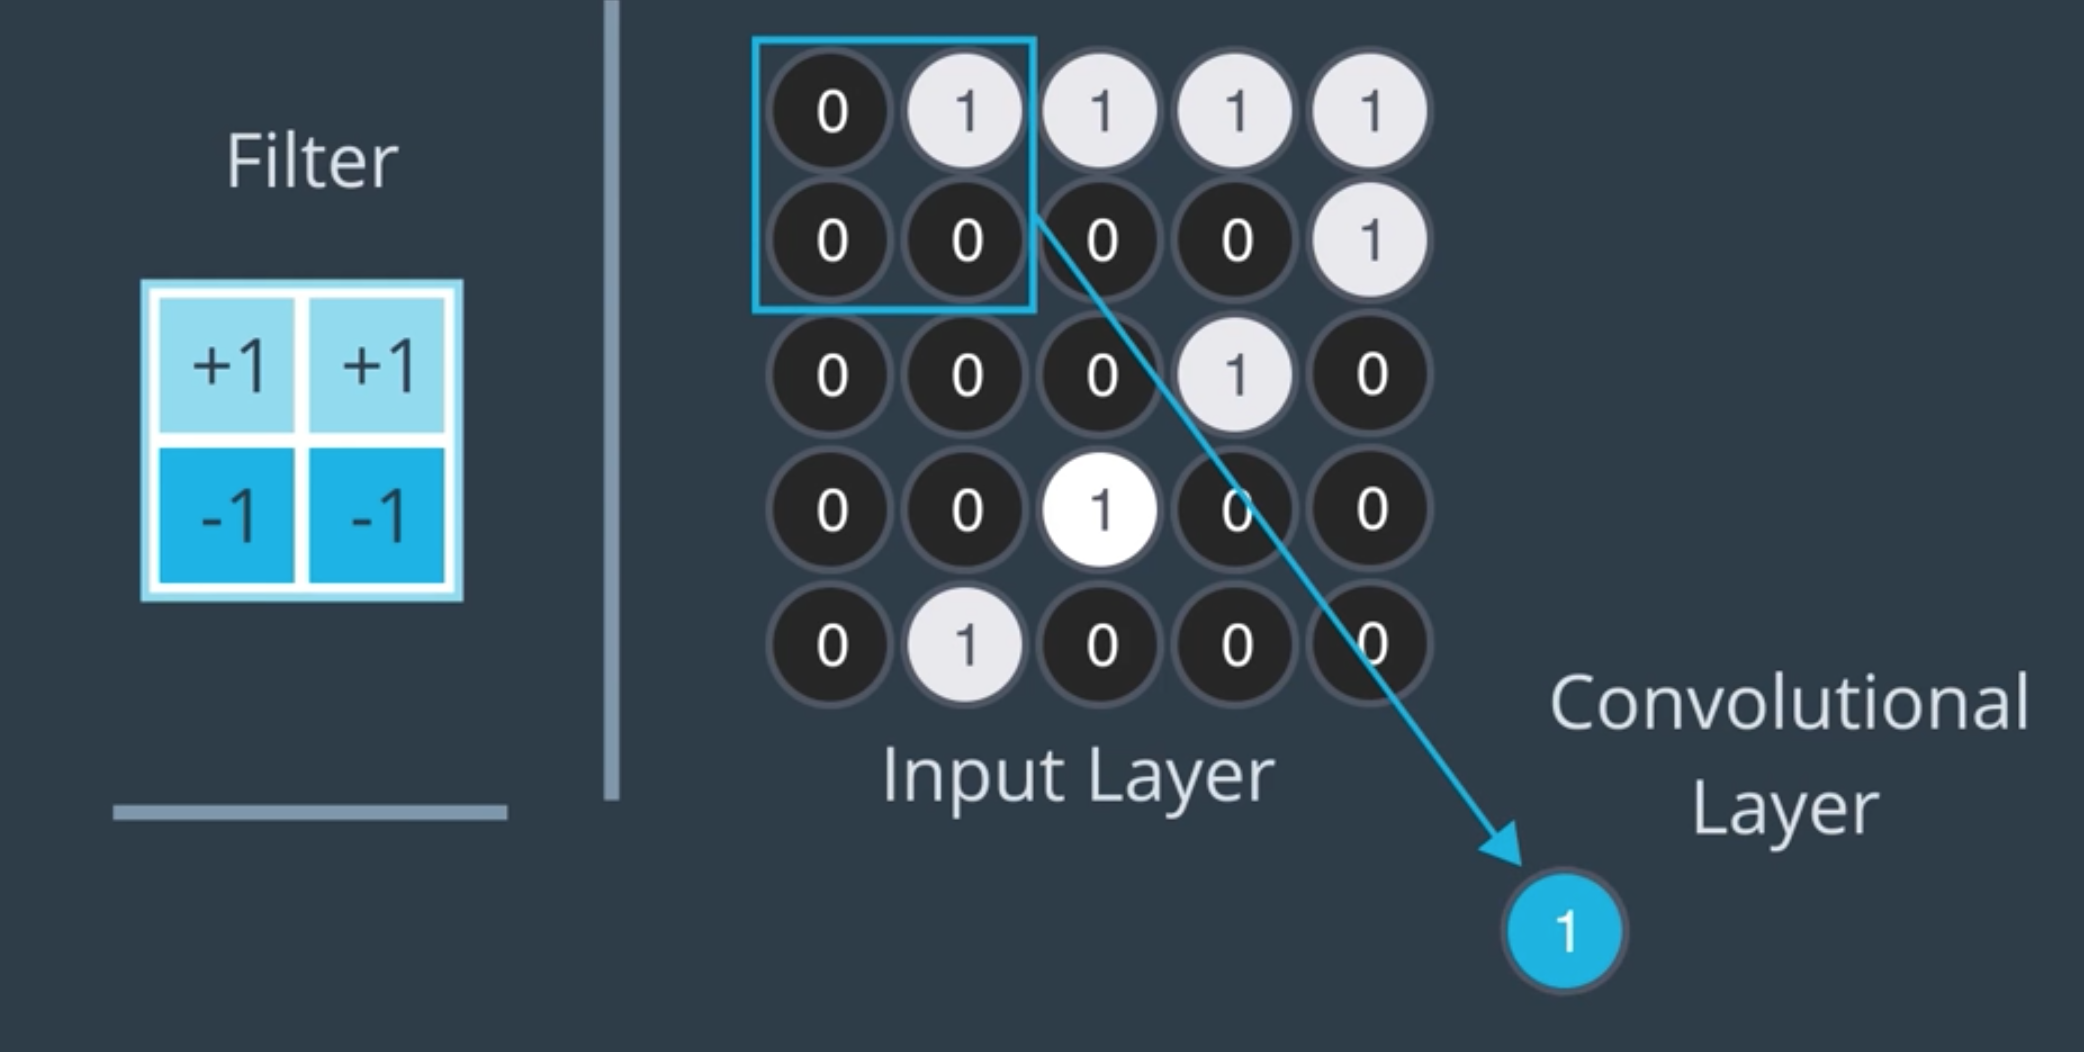
\includegraphics[width=0.75\linewidth]{img//cnn//depth/stride1.png}
\captionof{figure}{5x5 grey scale image}
\label{fig:stride1}

We have filter with the height and width of 2 and the stride is also 2. We start with the filter in the top left corner of the image \autoref{fig:stride1} and calculate the value for the first node in the convolutional layer.


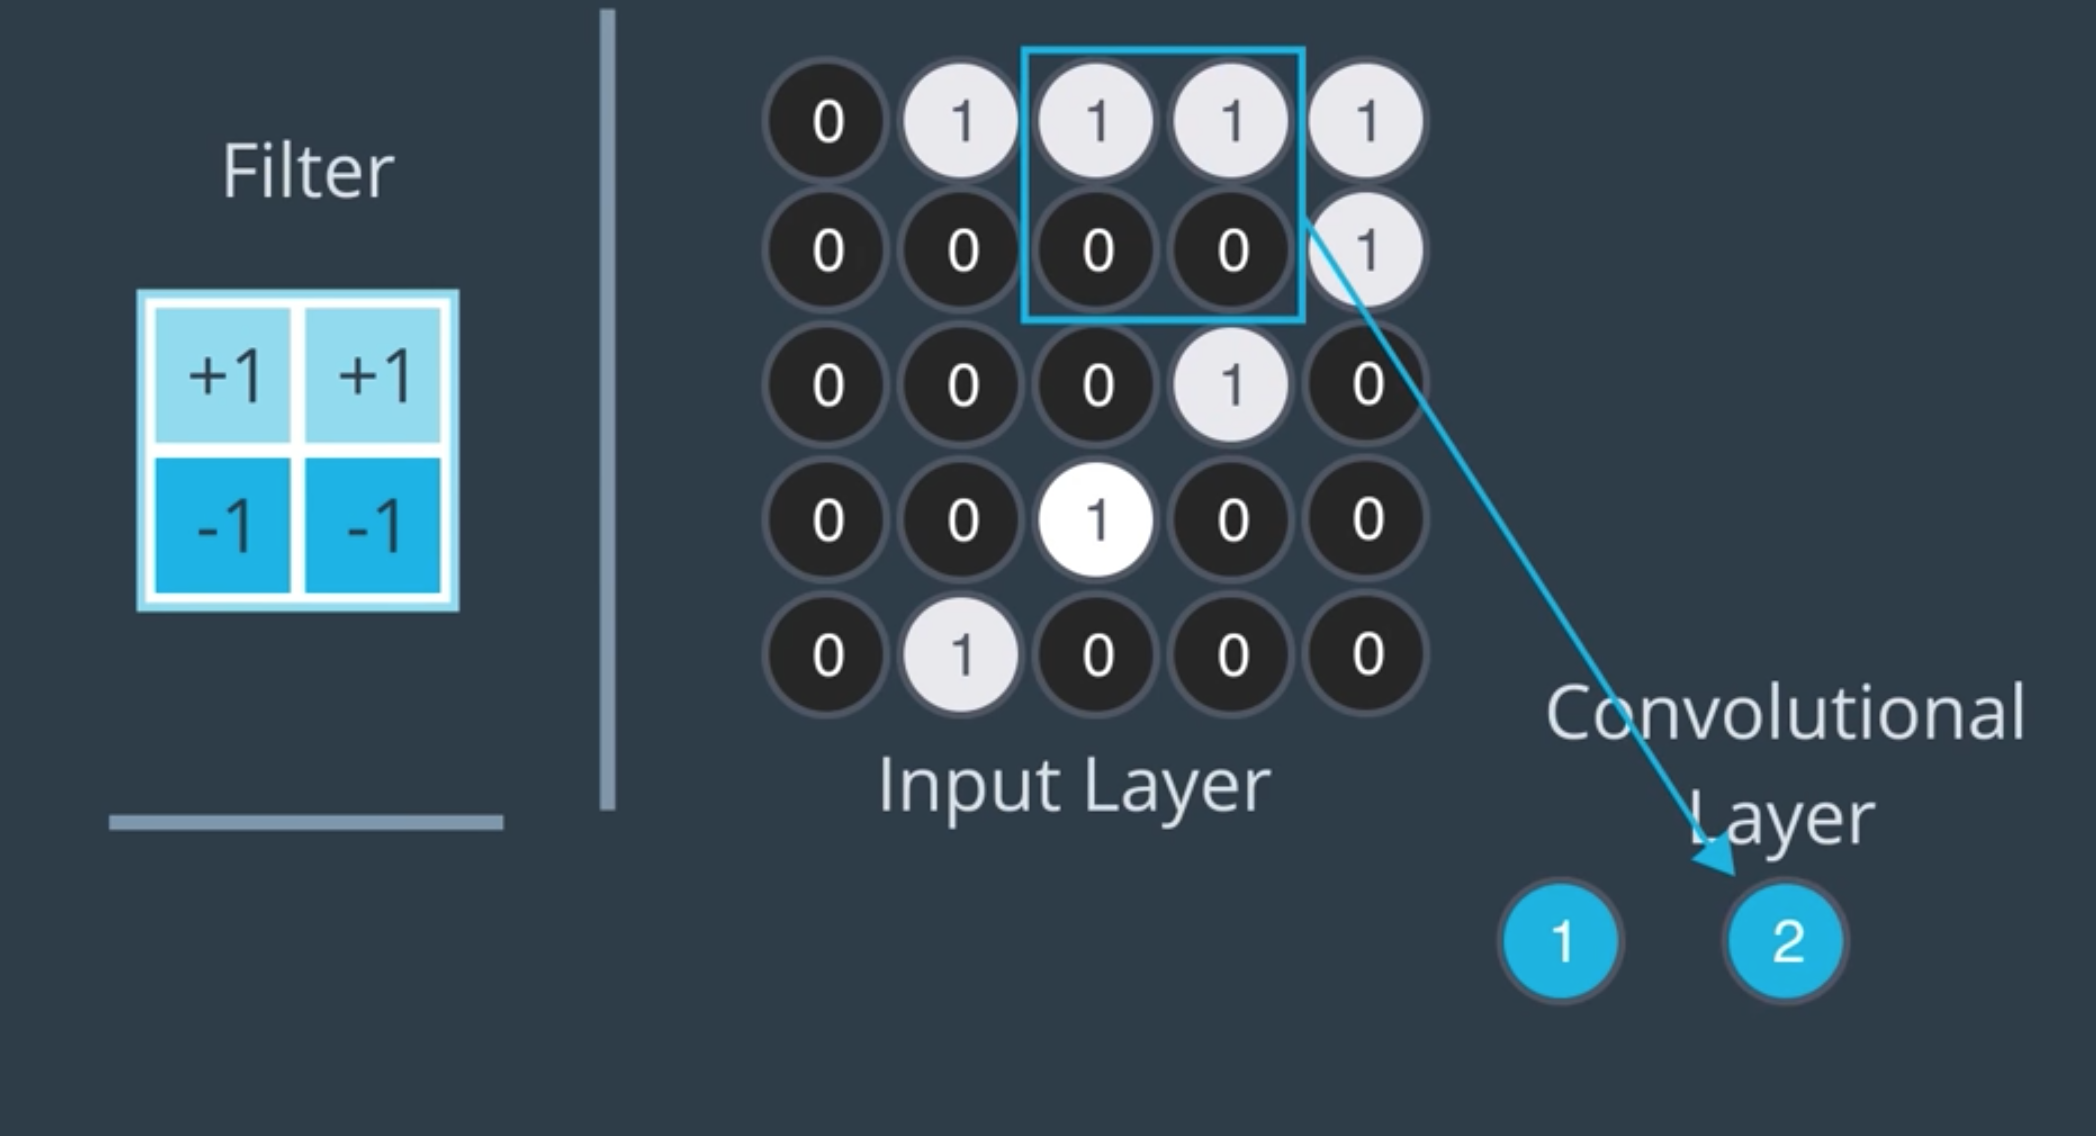
\includegraphics[width=0.75\linewidth]{img//cnn//depth/stride2.png}
\captionof{figure}{ }
\label{fig:stride2}

We then move the filter 2 units to the right and do the same (see \autoref{fig:stride2}).

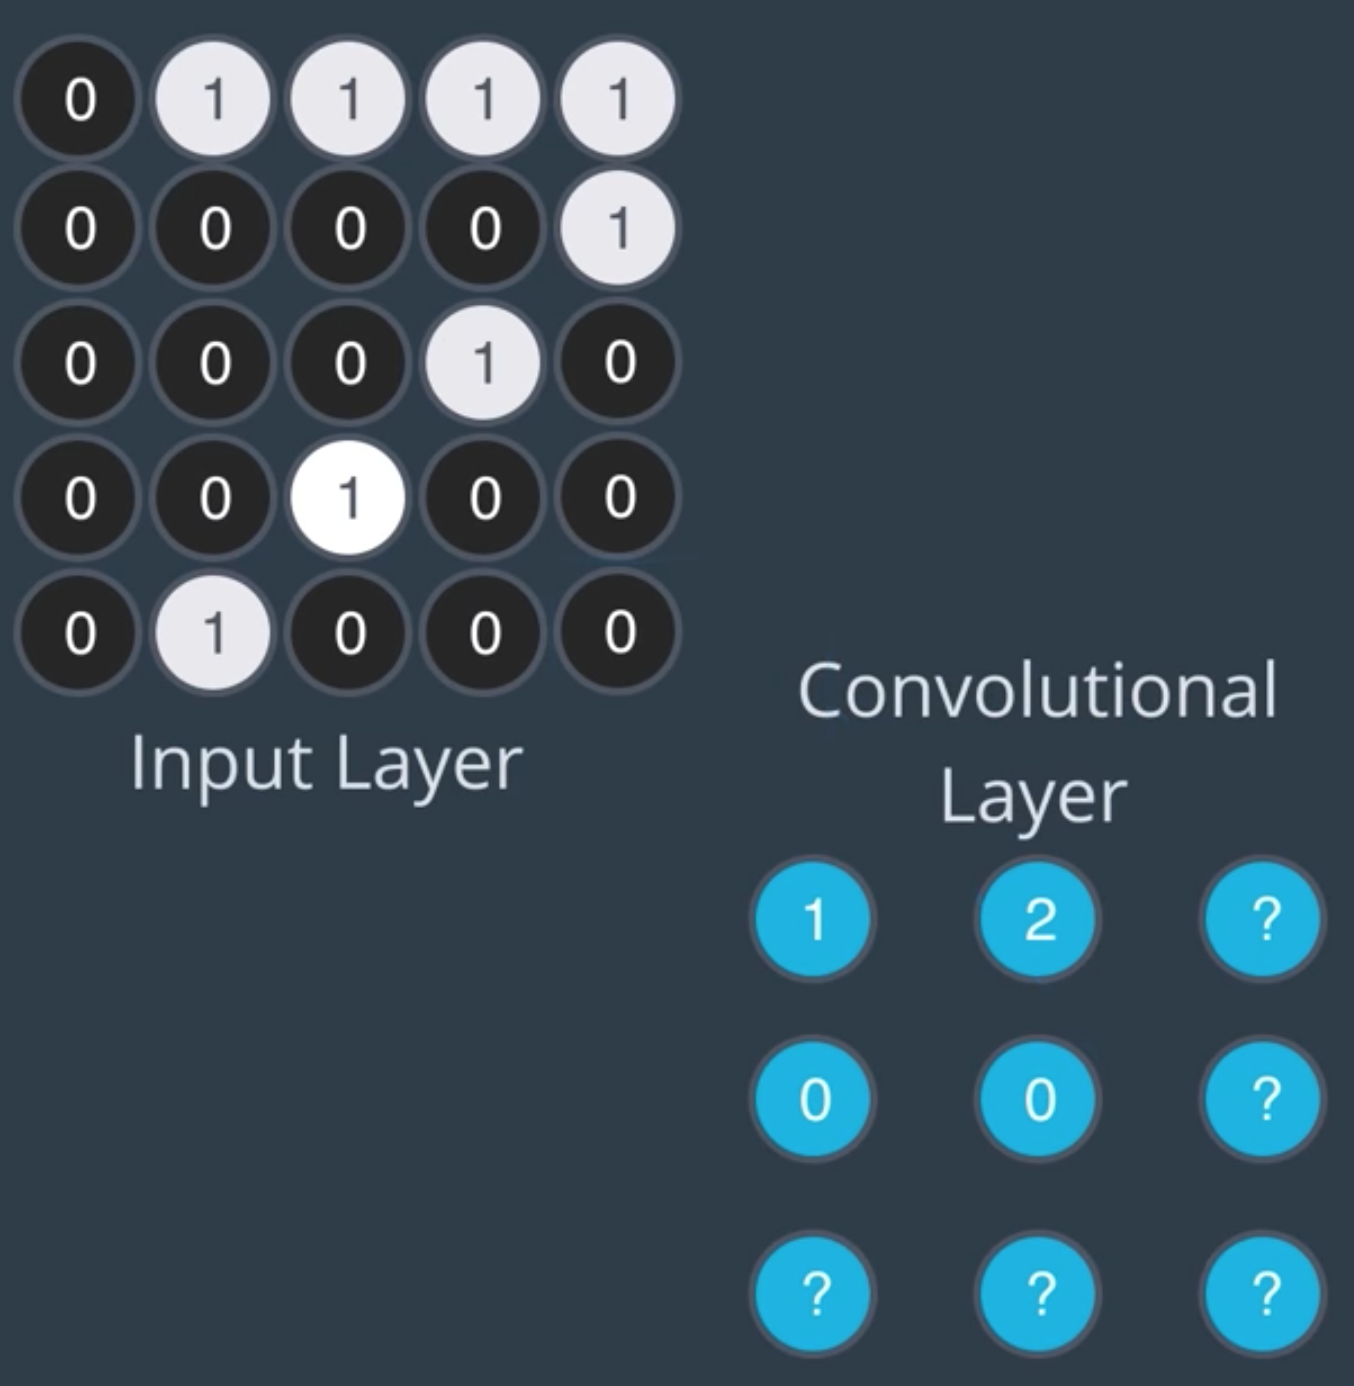
\includegraphics[width=0.75\linewidth]{img//cnn//depth/stride3.png}
\captionof{figure}{ }
\label{fig:stride3}

But when we move the filter 2 more units to the right, the filter extends outside the image. What do we do now? Do we still want to keep the corresponding convolutional node? For now, let's just populate the places where the filter extends outside with a question mark and proceed as planned (see \autoref{fig:stride3}). \newline

So now, how do we deal with these nodes where the filter extended outside the image? 

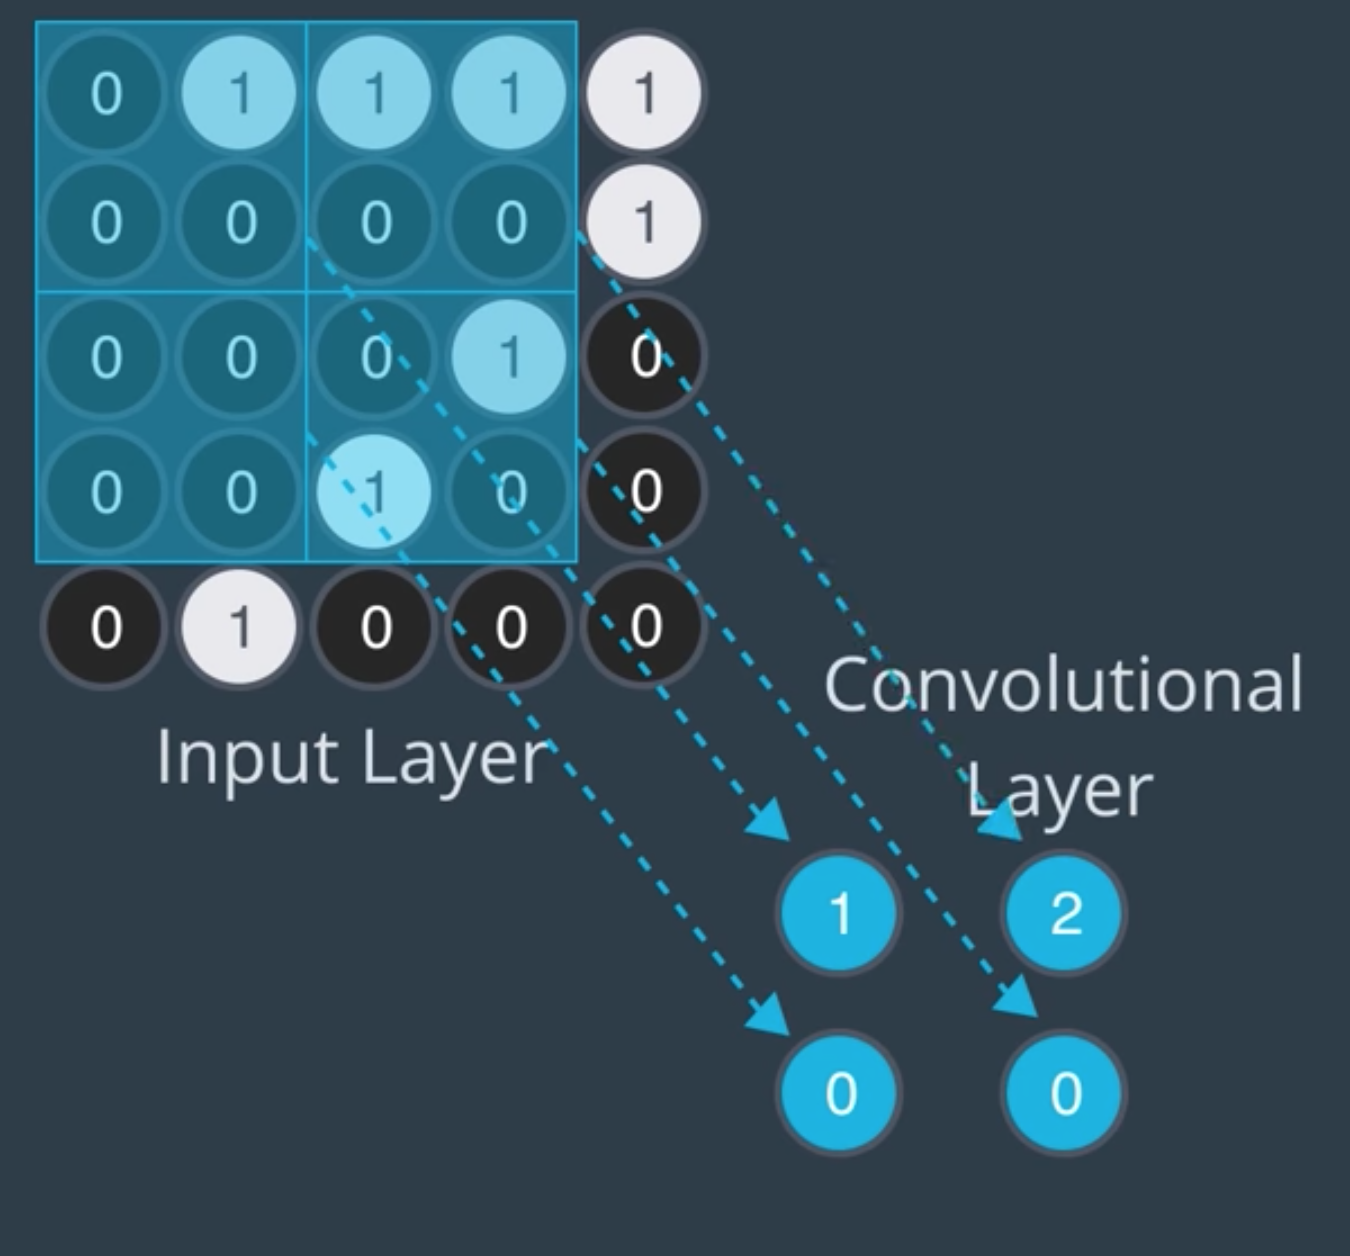
\includegraphics[width=0.75\linewidth]{img//cnn//depth/stride4.png}
\captionof{figure}{ }
\label{fig:stride4}

We could as a first option, just get rid of them. Note that if we choose this option, it is possible that our convolutional layer has no information about some regions of the image. This is the case for the right and bottom edges of the image in \autoref{fig:stride4}.

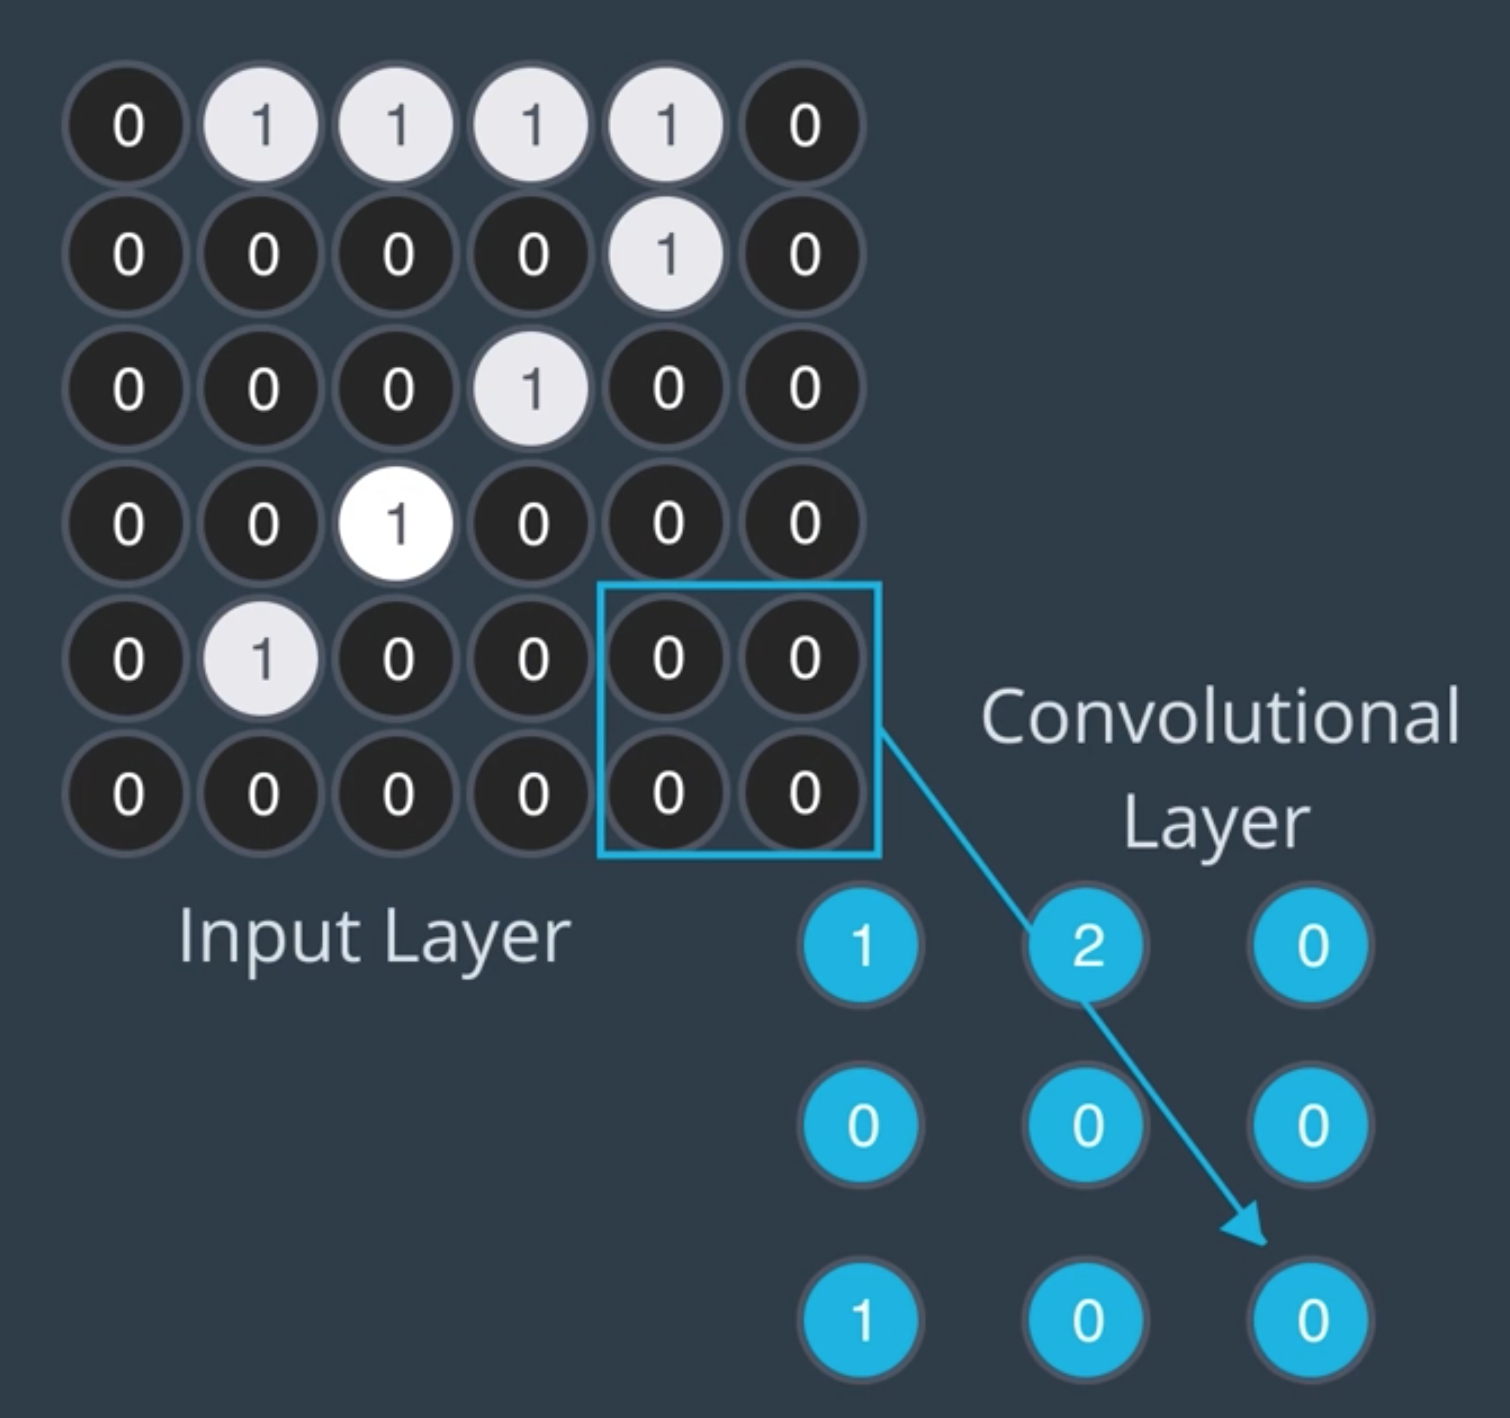
\includegraphics[width=0.75\linewidth]{img//cnn//depth/stride5.png}

As a second option, we could plan ahead for this case by padding the image with zeros to give the filter more space to move.
Now, when we populate the convolutional layer, we get contributions from every region in the image.

\subsection{Padding, Stride, Input and Output Size}

\textbf{Padding:} Expanding the size of an image by adding pixels at its border\newline

\textbf{Stride:} Amount by which a filter slides over an image.\newline

In PyTorch, the \lstinline|Conv2d| layer allows for an arbitrary amount of padding.\newline

Let's consider the first convolutional layer in a CNN, and let's assume that the input images are 5x5x1 (height of 5, width of 5, and grayscale) to make our math easier.\newline

We can for example define a first convolutional layer with 3 input channels (corresponding to the RGB of the image), 16 feature maps (also called output channels), a 3x3 kernel, and stride 1. This is defined in PyTorch as \lstinline{nn.Conv2d(3, 16, kernel_size=3, padding=0)}. We can visualize how one filter operates with the following animation:\newline


\href{run:./img/cnn/depth/i5-k3-s1-p0.gif}{3x3 Convolution on 5x5 Input with Stride 1 and No Padding}\newline
%\includegraphics[width=0.5\linewidth]{img//cnn//depth/i5-k3-s1-p0.gif}
%\captionof{figure}{3x3 Convolution on 5x5 Input with Stride 1 and No Padding}

As we can clearly see, the kernel fits in the image only 3 times per row, thus the output feature map is \(3 \times 3\). \newline

In many cases it is a good idea to keep the input size and the output size the same. Sometimes it is even necessary, as we will see in a different lesson when we talk about skip connections. In this particular case, we just need to add a padding of 1: \lstinline{nn.Conv2d(3, 16, kernel_size=3, padding=1)} (we will see later the different strategies to fill those values). This is the result:\newline

\href{run:./img/cnn/depth/same-padding-no-strides.gif}{3x3 convolution with padding 1 and stride 1. Input size and output size are the same.} \newline
% \includegraphics[width=0.5\linewidth]{img//cnn//depth/same-padding-no-strides.gif}
% \captionof{figure}{3x3 convolution with padding 1 and stride 1. Input size and output size are the same.}

What happens if instead of a 3x3 kernel we consider a 5x5 kernel? Obviously, without padding, the kernel would only fit once in the image. If we add a padding of 1, the kernel will fit 9 times in total and produce an image that is 3x3. \newline

\href{run:./img/cnn/depth/i5-k5-s1-p1.gif}{5x5 Convolution on 5x5 Input Image with Stride 1 and Padding 1} \newline
% \includegraphics[width=0.5\linewidth]{img//cnn//depth/i5-k5-s1-p1.gif}
% \captionof{figure}{5x5 Convolution on 5x5 Input Image with Stride 1 and Padding 1}

If we want our 5x5 convolution to produce the same size as the input, we have to use a padding of 2 this time: \newline

\href{run:./img/cnn/depth/i5-k5-s1-p2.gif}{5x5 convolution on 5x5 input image with stride 1, padding 2. Input and output have same size.} \newline
% \includegraphics[width=0.5\linewidth]{img//cnn//depth/i5-k5-s1-p2.gif}
% \captionof{figure}{5x5 convolution on 5x5 input image with stride 1, padding 2. Input and output have same size.}


\paragraph{Now Let's Consider Strides Larger than 1}

For a 5x5 input, a 3x3 kernel, a padding of 0, and a stride of 2 we have: \newline

\href{run:./img/cnn//epth/i5-k3-s2-p0.gif}{3x3 Convolution on 5x5 Input Image with Stride 2 and Padding 0} \newline
% \includegraphics[width=0.5\linewidth]{img//cnn//depth/i5-k3-s2-p0.gif}
% \captionof{figure}{3x3 Convolution on 5x5 Input Image with Stride 2 and Padding 0}

The kernel fits only 2 times per row, for a total output size of 2x2. If we want to have the output size equal to the input size we need to use a padding of 3 this time, but this does not make much sense: \newline

\href{run:./img/cnn/depth/i5-k3-s2-p3.gif}{3x3 Convolution on 5x5 Image with Stride 2 and Padding 2} \newline
% \includegraphics[width=0.5\linewidth]{img//cnn//depth/i5-k3-s2-p3.gif}
% \captionof{figure}{3x3 Convolution on 5x5 Image with Stride 2 and Padding 2}

Indeed, there are some pixels in the output feature map that are the result of convolving the kernel with a region that is completely outside of the original image. That region contains no information! However, by now you get the idea of how things work and we can derive a rule to help us in the computation of kernel size, padding, and output dimension.

\subsubsection{Formula for Convolutional Layers}

After working through the examples above, can you figure out a formula relating the output size, input size, kernel size, stride, and padding? (Try it on your own before looking below!) \newline

In general we can link together the output size \verb|o|, the size of the input image \verb|i|, the size of the kernel \verb|k|, the stride \verb|s| , and the padding \verb|p| with this simple formula, which is very useful when you are creating your own architectures:
\[o = \Bigg[\frac{i + 2p - k}{s}\Bigg] + 1 \]
\captionof{figure}{Simple Formula for Convolutional Layers}


\subsubsection{Quiz Question}

Use the formula we just provided to compute the expected output size for a convolution with kernel size 8x8, padding 3, and stride 2, applied on an image with an input size of 32x32.

\begin{itemize}
    \item \textbf{16x16}
    \item 32x32
    \item 15x15
\end{itemize}

\subsubsection{PyTorch Shortcuts}

In PyTorch you can also use \lstinline{padding="same"} or \lstinline{padding="valid"} instead of providing explicit numbers for the padding. The \lstinline{same} padding instructs PyTorch to automatically compute the amount of padding necessary to give you an output feature map with the same shape as the input. Note this option only works if you are using a stride of 1. The\lstinline{valid} padding is equivalent to using a padding of 0.

\subsection{Types of Padding}

As we have seen in the video there are different strategies to fill the padding pixels. The most obvious one is to fill them with zero (the default in PyTorch). However, the \lstinline{nn.Conv2d} layer in Pytorch also supports other options, illustrated by the following images:

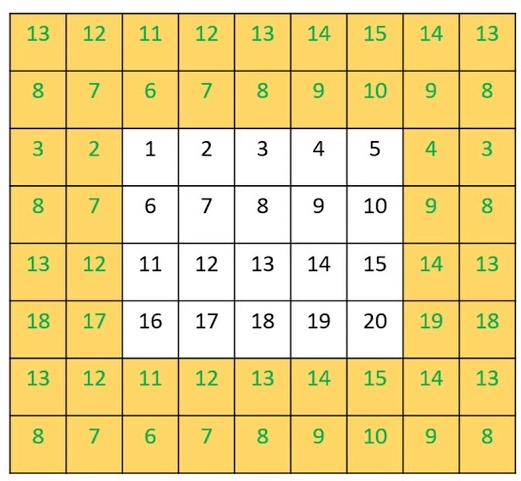
\includegraphics[width=0.75\linewidth]{img//cnn//depth/reflection-padding.jpeg}
\captionof{figure}{$padding\_mode='reflect'$: padding pixels filled with copies of values in input image taken in opposite order, in a mirroring fashion}

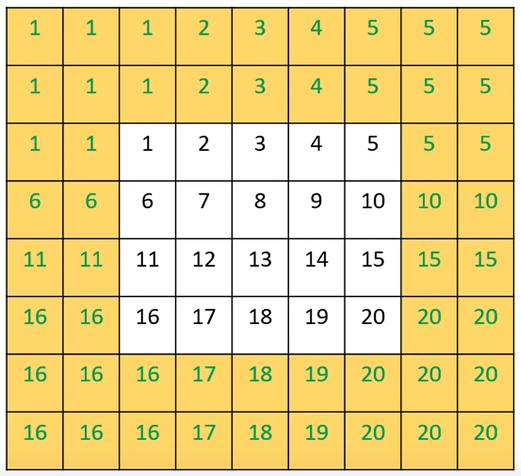
\includegraphics[width=0.75\linewidth]{img//cnn//depth/replicatepadding.jpeg}
\captionof{figure}{$padding\_mode='replicate'$: padding pixels filled with value of closest pixel in input image}

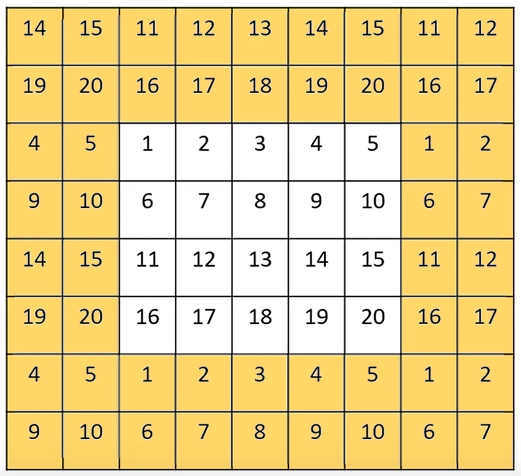
\includegraphics[width=0.75\linewidth]{img//cnn//depth/circularpadding.jpeg}
\captionof{figure}{$padding\_mode='circular'$: like reflect mode, but image is first flipped horizontally and vertically}

The zero-padding strategy is by far the most common, but these other strategies are adopted in some architectures and you can definitely experiment with them to see if they make any difference with respect to the zero-padding.


\section{Pooling Layers}
\href{https://www.youtube.com/watch?v=zTQsln05VqA&ab_channel=Udacity}{Youtube}\newline

You have previously learned about Max Pooling layers on a 1-channel image. Let's review that concept in the case of RGB images (3 channels). \newline

A convolutional layer is a stack of feature maps where we have one feature map for each filter.
A complicated dataset with many different object categories will require a large number of filters, each responsible for finding a pattern in the image. More filters means a bigger stack, which means that the dimensionality of our convolutional layers can get quite large. Higher dimensionality means we will need to use more parameters which can lead to over-fitting. Thus, we need a method for reducing this dimensionality. \newline

This is the role of pooling layers within a convolutional neural network. Max pooling layers will take a stack of feature maps as input.

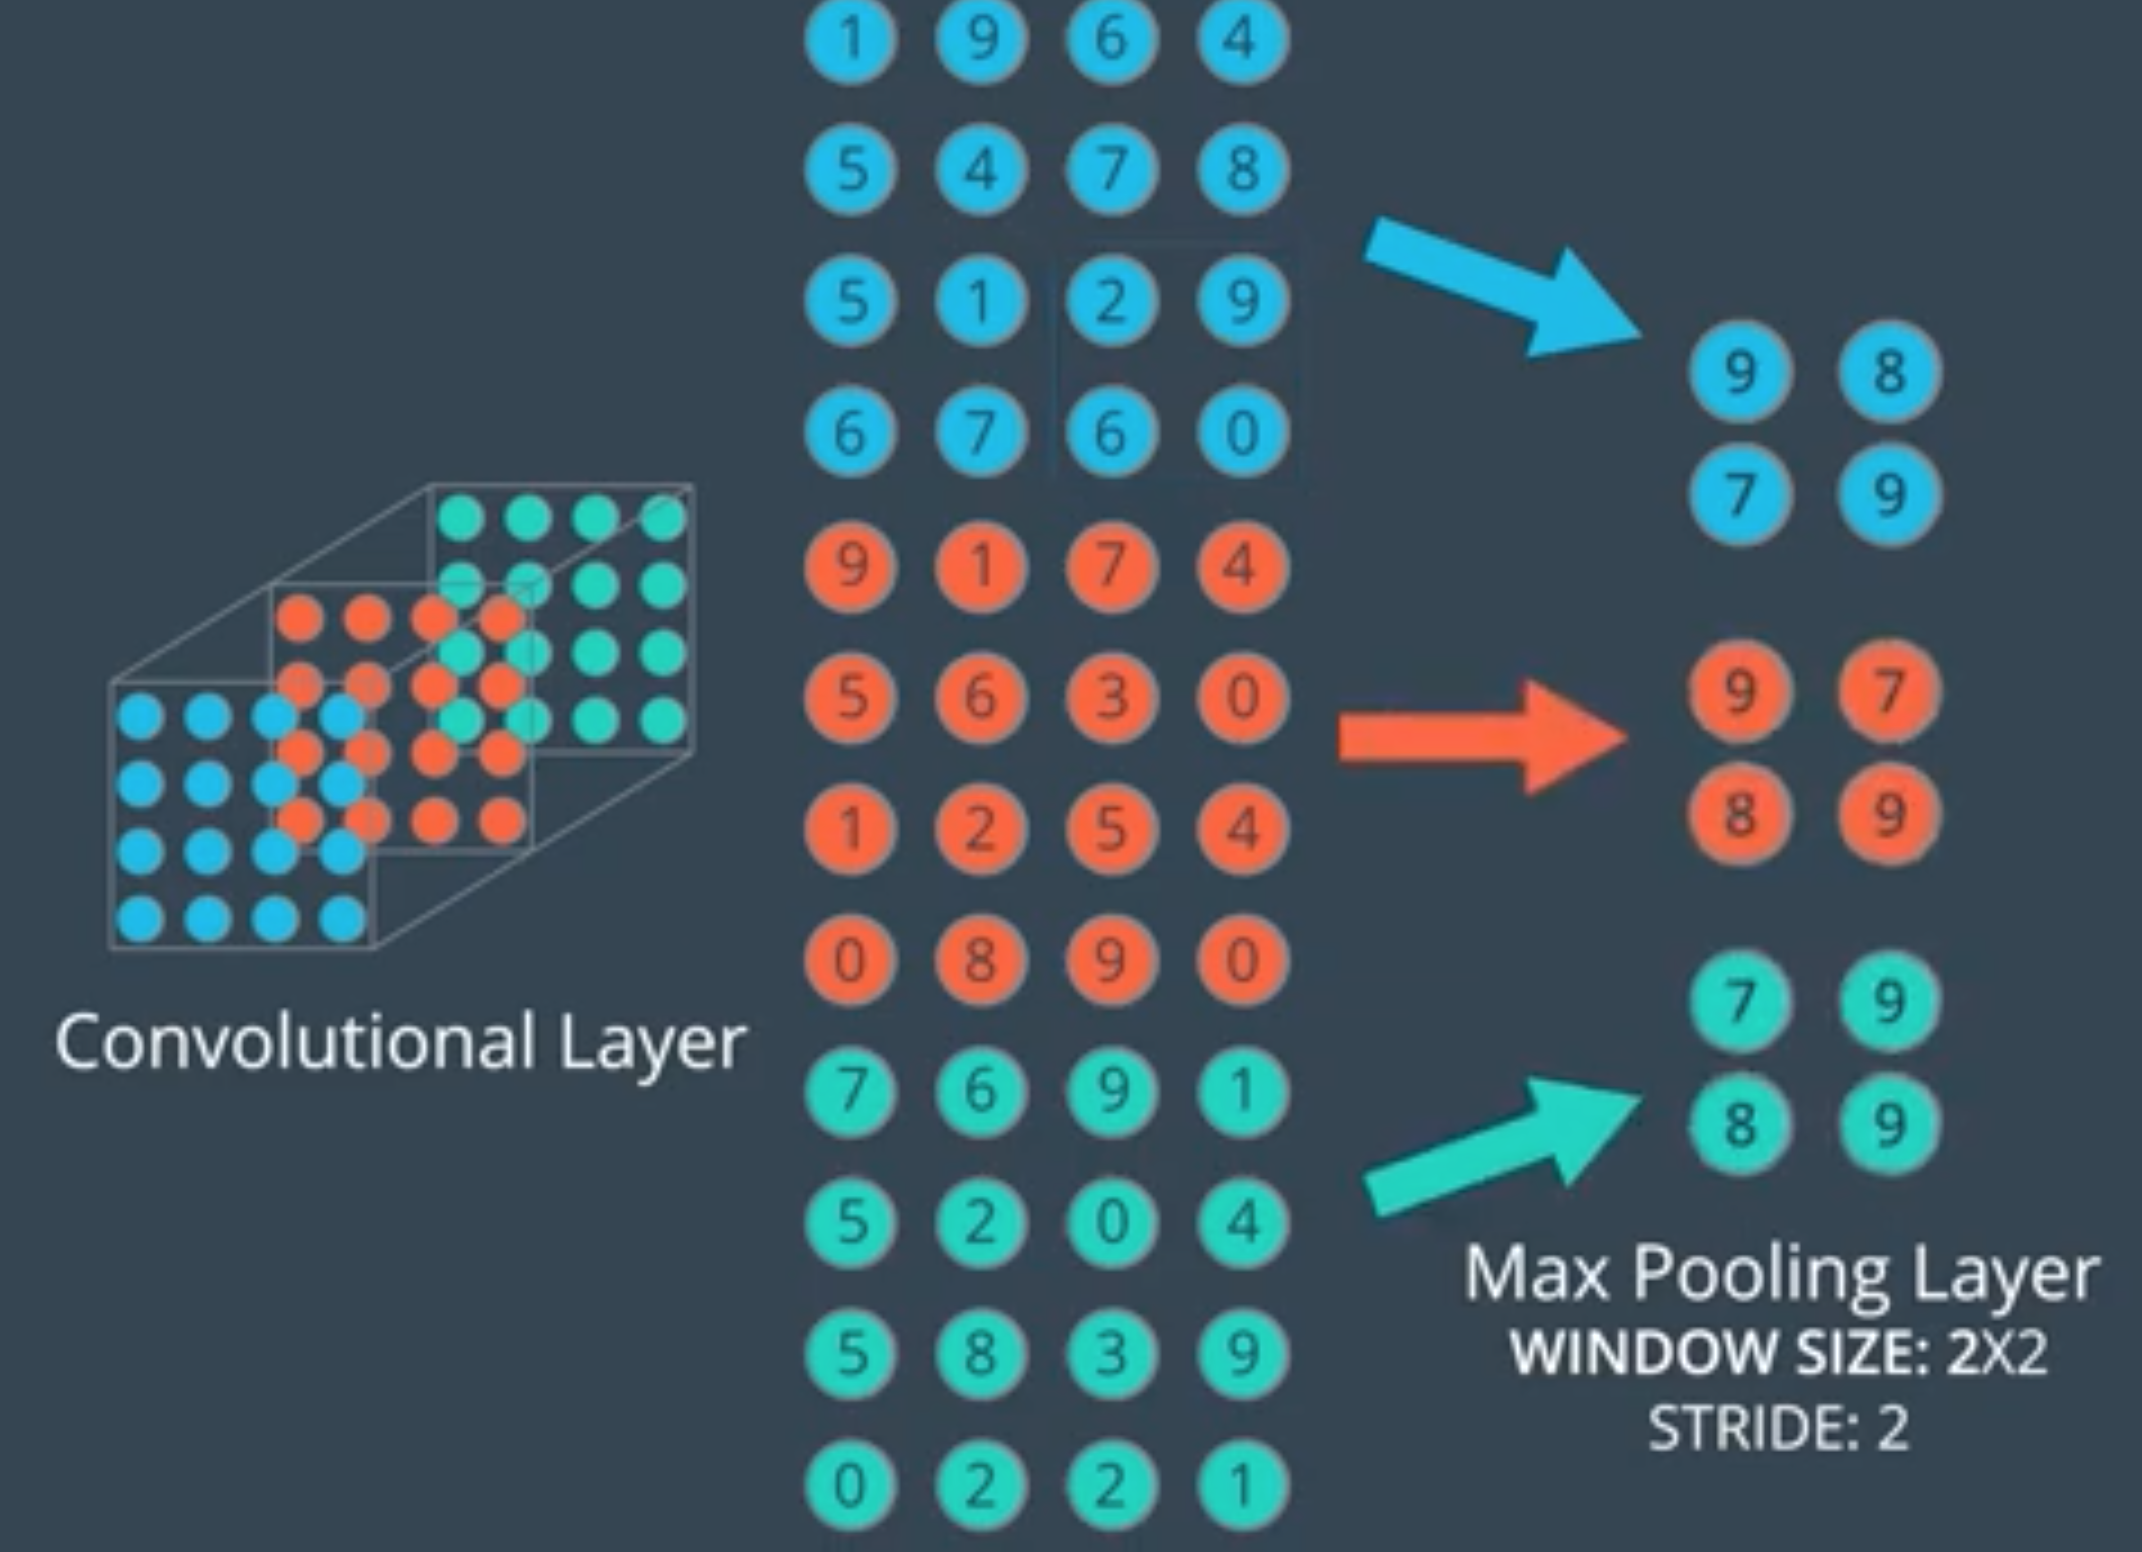
\includegraphics[width=1\linewidth]{img//cnn//depth/image_maxpooling.png}
\captionof{figure}{ }
\label{fig:image_maxpooling}

In \autoref{fig:image_maxpooling} we've enlarged and visualized all three of the feature maps. To construct the max pooling layer we will work with each feature map separately.
Let's begin with the first feature map. We start with our window in the top left corner of the image. The value of the corresponding node in the max pooling layer is calculated by just taking the maximum of the pixels contained in the window. In this case, we had a 1, 9, 5, and 4 in our window, so 9 was the maximum.
If we continue this process and do it for all of our feature maps, the output is a stack with the same number of feature maps,
but each feature map has been reduced in width and height. In this case, the width and height are half of that of the previous convolutional layer.

\subsection{Other Kinds of Pooling}

You now know how the Max Pooling layer works, but there are other types of pooling layers. One we can introduce now is called Average Pooling.

\subsubsection{Average Pooling}

This works similarly to the Max Pooling layer, but instead of taking the maximum for each window, we take the mean average of all the values in the window.

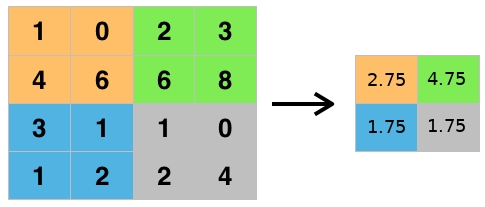
\includegraphics[width=0.75\linewidth]{img//cnn//depth/average-pooling.jpeg}
\captionof{figure}{Average Pooling}

Average Pooling is not typically used for image classification problems because Max Pooling is better at noticing the most important details about edges and other features in an image, but you may see average pooling used in applications for which \textit{smoothing} an image is preferable. \newline

Sometimes, Average Pooling and Max Pooling are used together to extract both the maximum activation and the average activation.

\section{Pooling Layers in PyTorch}

\subsection{Max Pooling Layers in PyTorch}

To create a pooling layer in PyTorch, you must first import the necessary module:

\begin{lstlisting}
from torch import nn
\end{lstlisting}
Then you can define the layer as:
\begin{lstlisting}
nn.MaxPool2d(kernel_size, stride)
\end{lstlisting}
You must pass the following arguments:

\begin{itemize}
    \item \lstinline{kernel_size} - The size of the max pooling window. The layer will roll a window of this size over the input feature map and select the maximum value for each window.
    \item \lstinline|stride| - The stride for the operation. By default the stride is of the same size as the kernel (i.e., \lstinline{kernel_size}).
\end{itemize}
There are some additional optional arguments that are rarely used, but could be helpful under certain circumstances. Please refer to the \href{https://pytorch.org/docs/stable/generated/torch.nn.MaxPool2d.html}{\textbf{PyTorch documentation on MaxPool2D.}}.

\subsection{Average Pooling Layer}

Similarly, an Average Pooling Layer can be created in this way:
\begin{lstlisting}
pooling = nn.AvgPool2d(window_size, stride)
\end{lstlisting}
where the parameters have the same meaning as for the Max Pooling layer.


\section{Quiz Question}

Can you match each term with its definition?

\begin{table}[!htbp]
    \centering
    \begin{tabular}{|c | c |}
    \hline 
        Definition & Term\\
        Size of the side of the convolutional kernel & kernel size\\
        Size of the window considered during pooling & window size\\
        Step size of the convolutional kernel or of the pooling window when moving over the input image & stride\\
        Border to add to an input image before the convolution operation is performed & padding\\
        \hline
    \end{tabular}
\end{table}

\section{Quiz Question}

Consider the following image for the this quiz question:

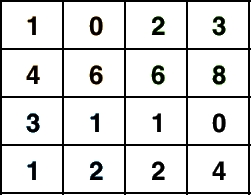
\includegraphics[width=0.5\linewidth]{img//cnn//depth/pooling-question.jpeg}

Consider the following layer: \lstinline{nn.MaxPooling(2, 2)}
What would be the result after applying this layer?

\begin{itemize}
    \item 6,6,8,6,6,8,3,2,4
    \item 1,2,1,0
    \item \textbf{6,8,3,4}
    \item 2.5, 4.75, 1.75, 1.75
\end{itemize}

\section{Quiz Question}

Let's consider a convolutional layer with \lstinline{in_channels=3}, \lstinline{out_channels=16}, \lstinline{kernel_size=5} and \lstinline{padding=2}. How many parameters does the layer have?
\begin{itemize}
    \item 1200
    \item \textbf{1216}
    \item 48
    \item 720
\end{itemize}

\section{Structure of a Typical CNN}
\href{https://www.youtube.com/watch?v=-e4kvl-8y_A&ab_channel=Udacity}{Youtube} \newline

In a typical CNN there are several convolutional layers intertwined with Max Pooling layers. The convolutional layers have more and more feature maps as you go deeper into the network, but the size of each feature map gets smaller and smaller thanks to the Max Pooling layer.

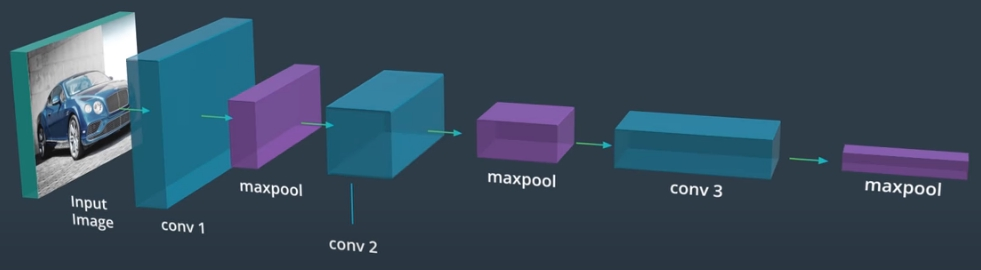
\includegraphics[width=1\linewidth]{img//cnn//depth/cnn-structure.jpeg}
\captionof{figure}{Structure of a Classical CNN}

This kind of structure goes hand in hand with the intuition we have developed in another lesson: as the signal goes deeper into the network, more and more details are dropped, and the content of the image is "abstracted." In other words, while the initial layers focus on the constituents of the objects (edges, textures, and so on), the deeper layers represent and recognize more abstract concepts such as shapes and entire objects


\section{CNN Structure and Layers in PyTorch: Recap}
\href{https://www.youtube.com/watch?v=smaw5GqRaoY&t=2s&ab_channel=Udacity}{Youtube} \newline

We want to classify an input image. There are a few ways we could go about this using a deep learning architecture.

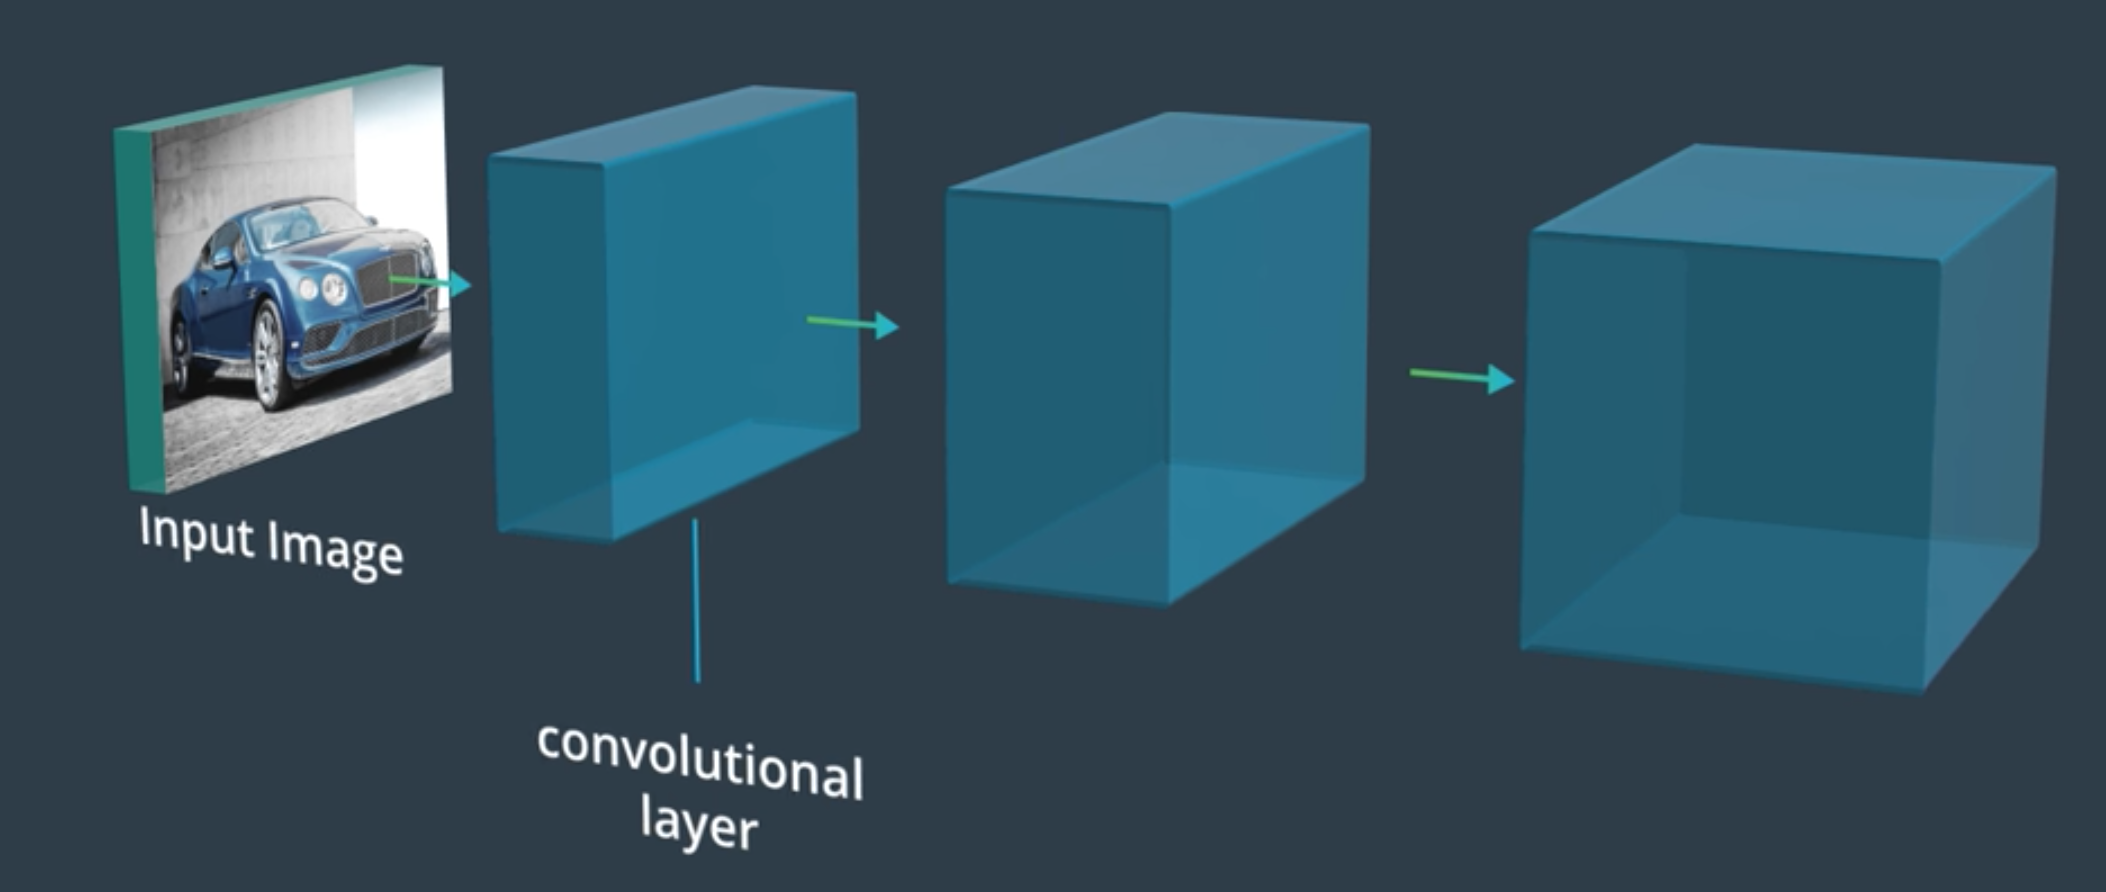
\includegraphics[width=0.75\linewidth]{img//cnn//depth/image6.png}

Consider following the input layer with a sequence of convolutional layers. This stack will discover hierarchies of spatial patterns in the image. The first layer of filters looks at patterns in the input image, the second looks at patterns in the previous convolutional layer, and so on. 

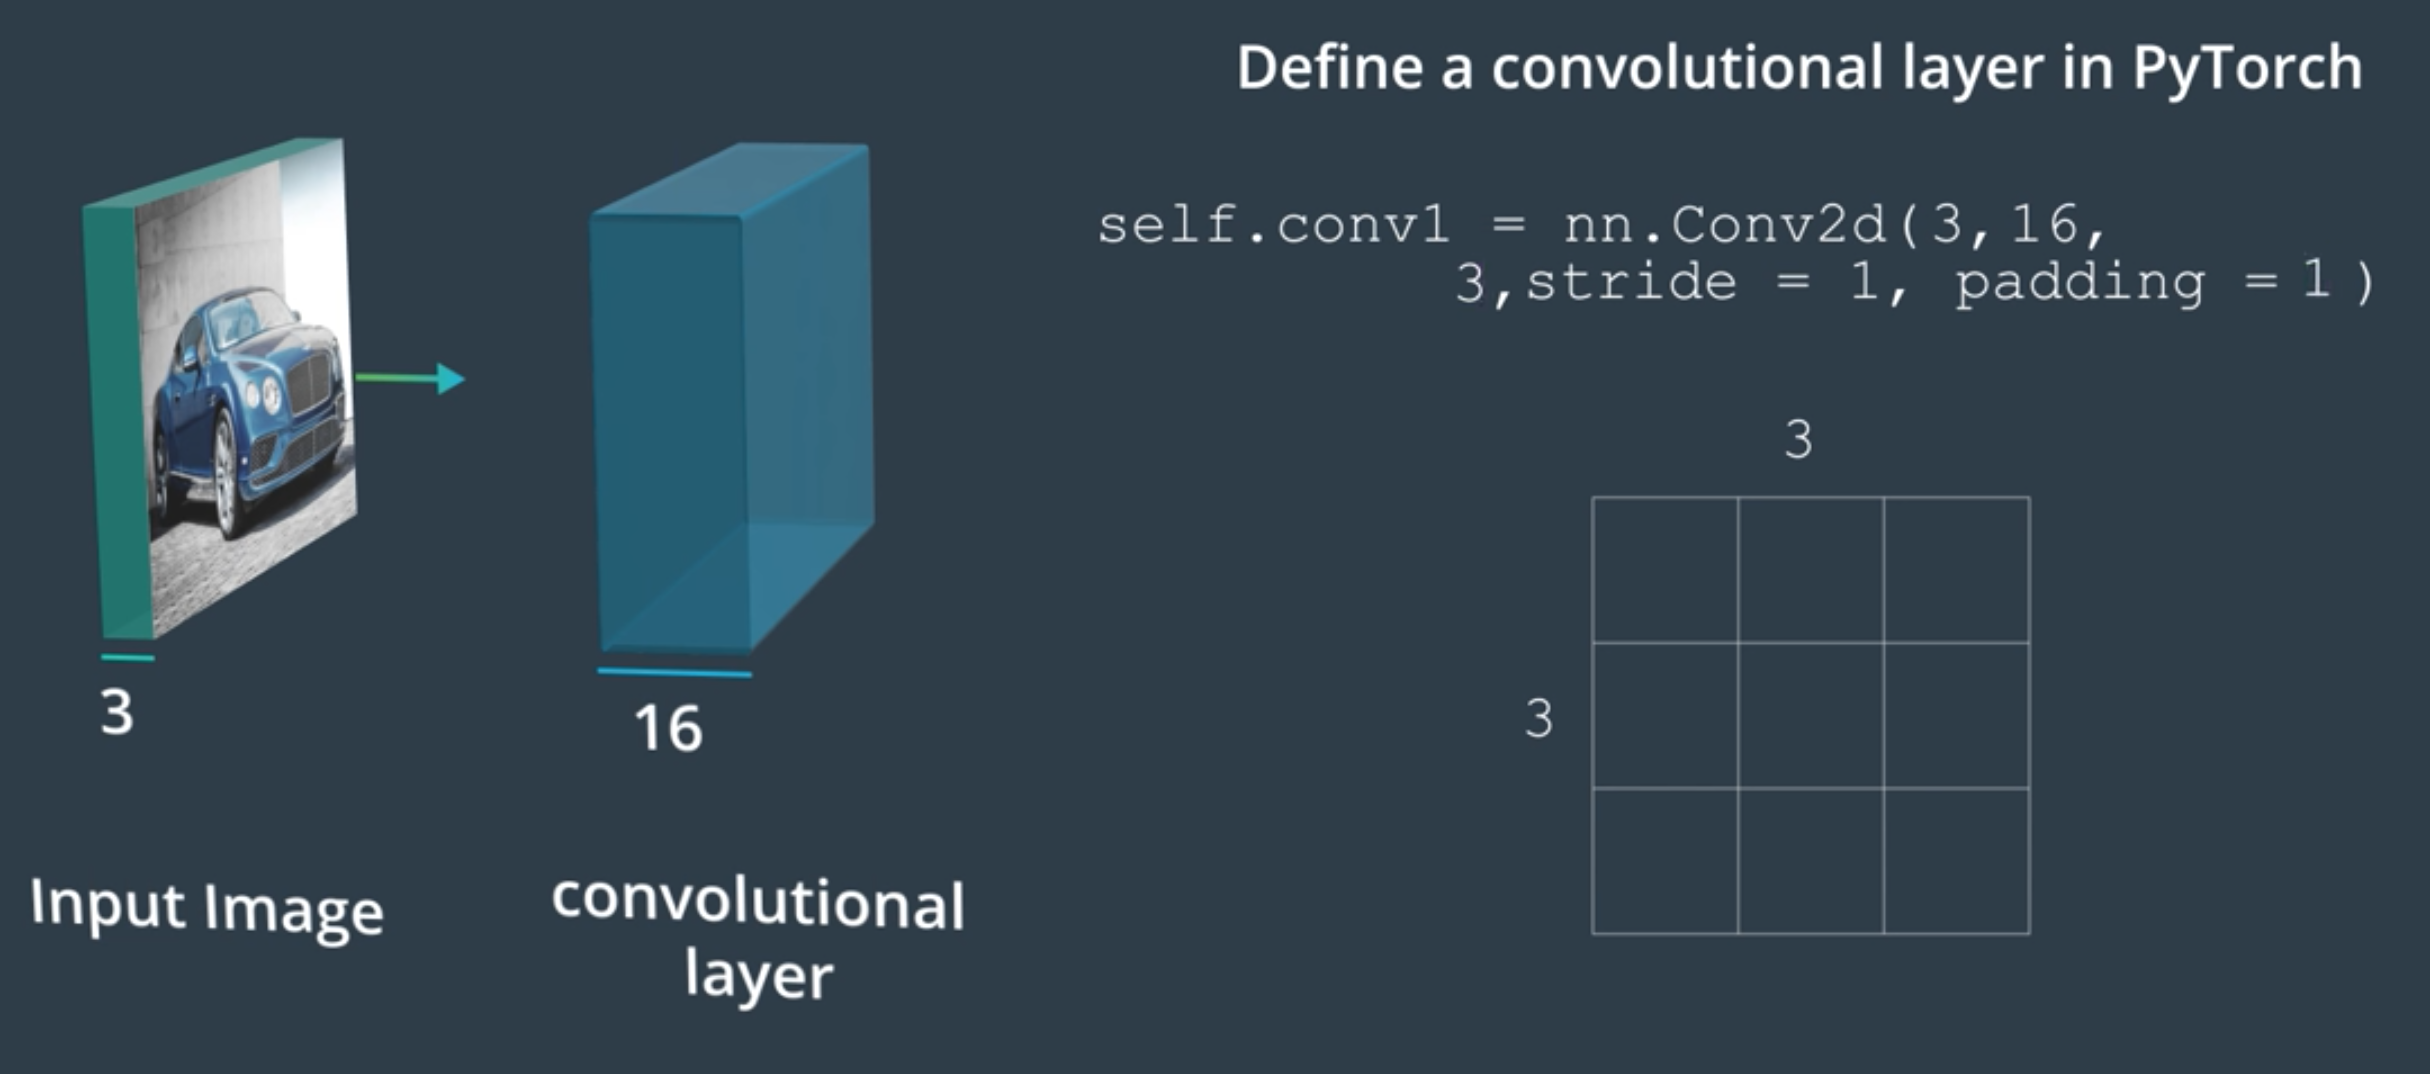
\includegraphics[width=0.75\linewidth]{img//cnn//depth/image7.png}

Each of the convolutional layers requires us to specify a number of hyperparameters. The first and second inputs to define a convolutional layer are simply the depth of the input and the desired depth of the output. The input depth of a color image will be 3 for the RGB channels,and we might want to produce 16 different filtered images in this convolutional layer. Next, we define the size of the filters that define a convolutional layer. These are often square and range from the size of \(2 \times 2\) at the smallest to up to a \(7x7\) or so for very large images. Here, we choose to use \(3 \times 3\) filters.
The stride is generally set to 1 and many frameworks will have this as the default value, so you may need to input this value.
As for padding, you may get better results if you set your padding such that a convolutional layer will have the same width and height as its input from the previous layer. In the case of a \(3 \times 3\) filter, which can almost center itself perfectly on an image but misses the border pixels by 1, this padding will be equal to 1. \newline

When deciding the depth or number of filters in a convolutional layer,
often we have a number of filters increase in sequence. So, the first convolutional layer might have 16 filters. The second second will see that depth as input and produce a layer with a depth of 32. The third will have a depth of 64 and so on. \newline

After each convolutional layer, we apply a ReLU activation function. If we follow this process, we have a method for gradually increasing the depth of our array without modifying the height and width. The input, just like all of the layers in this sequence, has a height and width of 32. But the depth increases from an input layers depth of 3 to 16 to 32 to 64. \textbf{We want to increase the depth, but we also want to decrease the height and width and discard some spatial information}. This is where \textit{max pooling layers} will come in. They generally follow every one or two convolutional layers in the sequence.

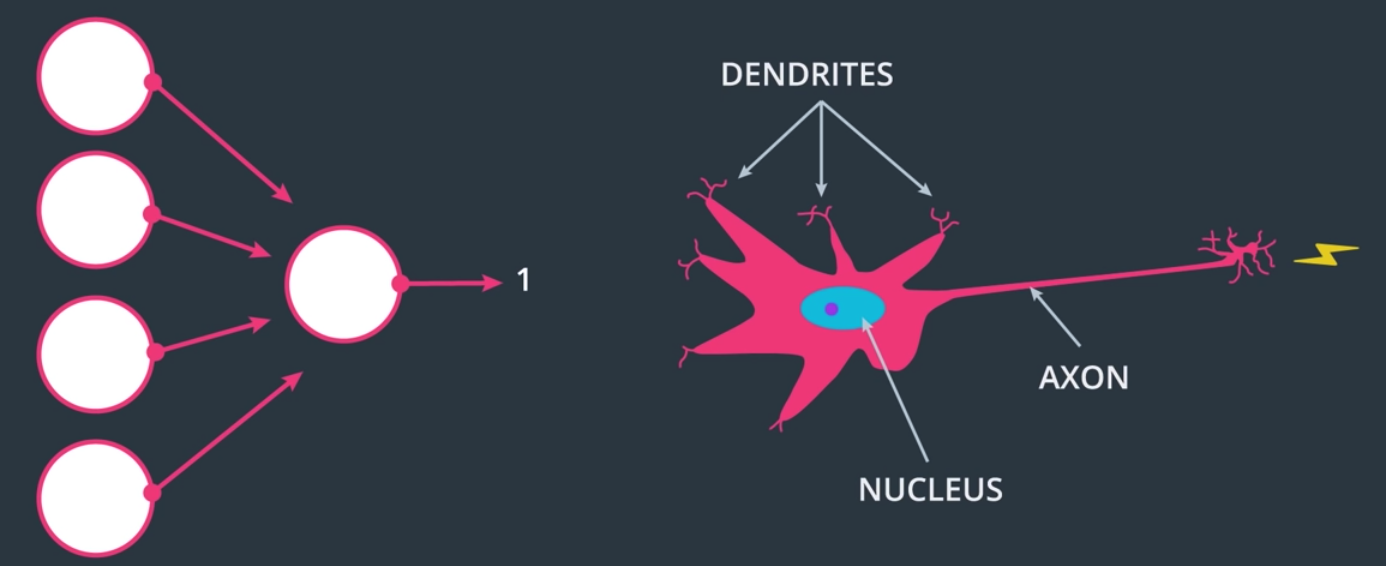
\includegraphics[width=0.75\linewidth]{img//cnn//depth/image.png}

Here's one such example with a max pooling layer after each convolutional layer.
To define a max pooling layers, you only need to define the filter size and stride. The most common setting will use filters of size 2 with a stride of 2. This has the effect of making the XY dimensions half of what they were from the previous layer.
In this way, the combination of convolutional and max pooling layers accomplishes our goal of attaining an array that's quite deep but small in the X and Y dimensions. \newline

Let's recap what we have learned so far about the typical structure of a CNN and the layers that constitute a CNN. \newline

The convolution part of a CNN is implemented in PyTorch by using the \lstinline{nn.Conv2d} layer for convolution and the \lstinline{nn.MaxPool2d} layer for max pooling. Stacking different blocks of convolution followed by pooling constitutes the typical structure of a simple CNN. Typically the sizes of the feature maps shrink as you go deeper into the network, while the channel count (i.e., the number of feature maps and filters) increases going deeper into the network, as shown below.


\section{Feature Vectors}
\href{https://www.youtube.com/watch?v=BzGasoPqzWY&t=1s&ab_channel=Udacity}{Youtube} \newline

The job of a convolutional neural network is to discover patterns contained in an image.
A sequence of layers is responsible for this discovery. The layers in a CNN convert an input image array into a representation that encodes only the content of the image. This is often called a \textbf{feature level representation of an image} or a \textbf{feature vector}. \newline

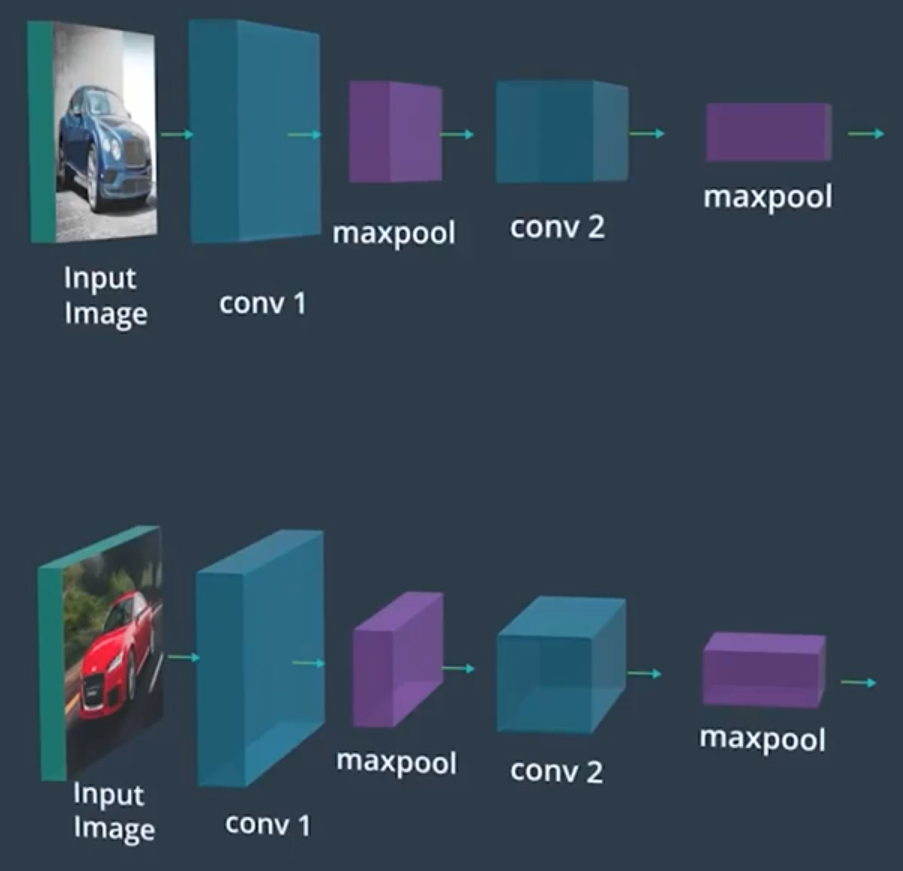
\includegraphics[width=1\linewidth]{img//cnn//depth/imagecar.png}

Take 2 input images that are both images of a car. Both are very different, and if I was to frame these pictures, the detail would be what makes them stylistically interesting. But for an image classifier, it only wants to know that these are both images of cars. When you look at how these images are transformed as they move through several layers of a CNN, the exact original pixel values matter less and less. The 2 transformed outputs should start to look much more similar to one another. Moving closer towards the idea that both are a car, rather than the details about what the cars look like.

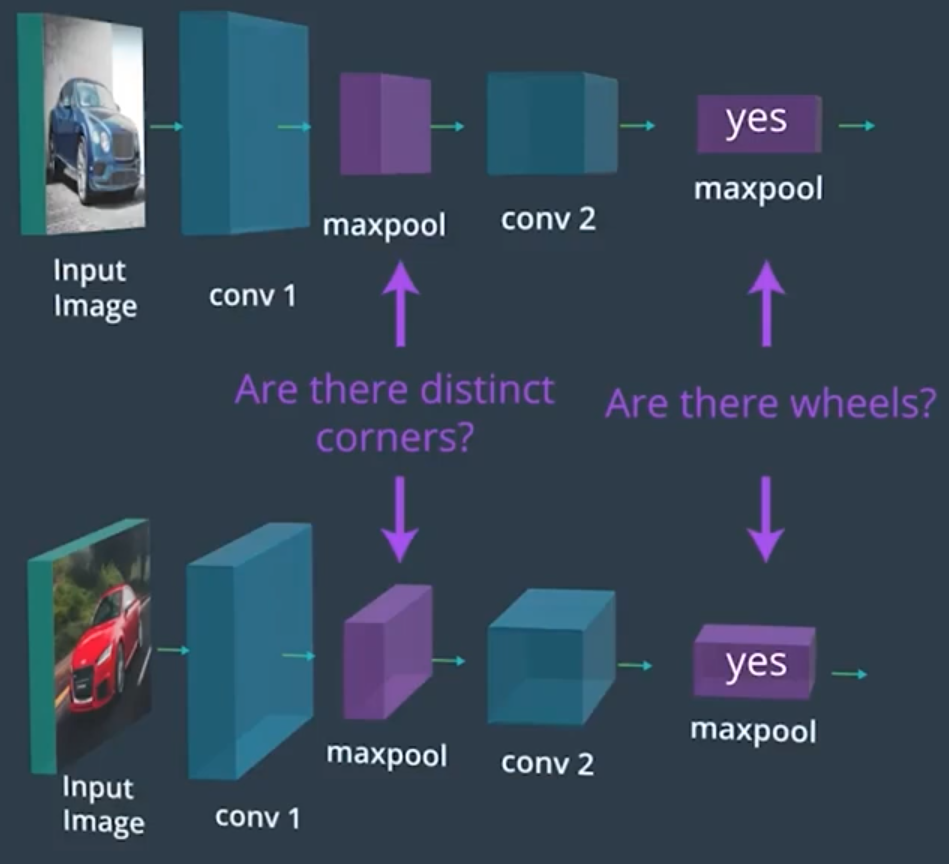
\includegraphics[width=1\linewidth]{img//cnn//depth/imagecar2.png}

Later layers in a CNN have discarded information about style and texture, and instead are pushed towards answering questions about general shape and about the presence of unique patterns,
like are there wheels in the image, are there eyes in the image, what about furry legs or tails? \newline

Once we get to a representation where the content of an image has been distilled like this,
we can flatten the array into a feature vector and feed it to one or more fully connected layers to determine what object is contained in the image.\newline

For instance, if wheels were found after the last max pooling layer, the feature vector will be able to reflect that, and the fully connected layer will transform that information to predict that a car is present in the image with higher probability.
If there were eyes, furry legs and a tail, then the output layer would take that information and deduce that a dog is likely present in the image.\newline

All of this understanding in the model is not pre-specified by us. It is learned by the model during training and through backpropagation that updates the weights that define
the filters and the weights in the fully connected layers. This architecture that we're specifying here just gives the model a structure that will allow it to train better. It has the potential to classify objects with greater accuracy.\newline

A classical CNN is made of two distinct parts, sometimes called the \textbf{backbone} and the \textbf{head,} illustrated below.

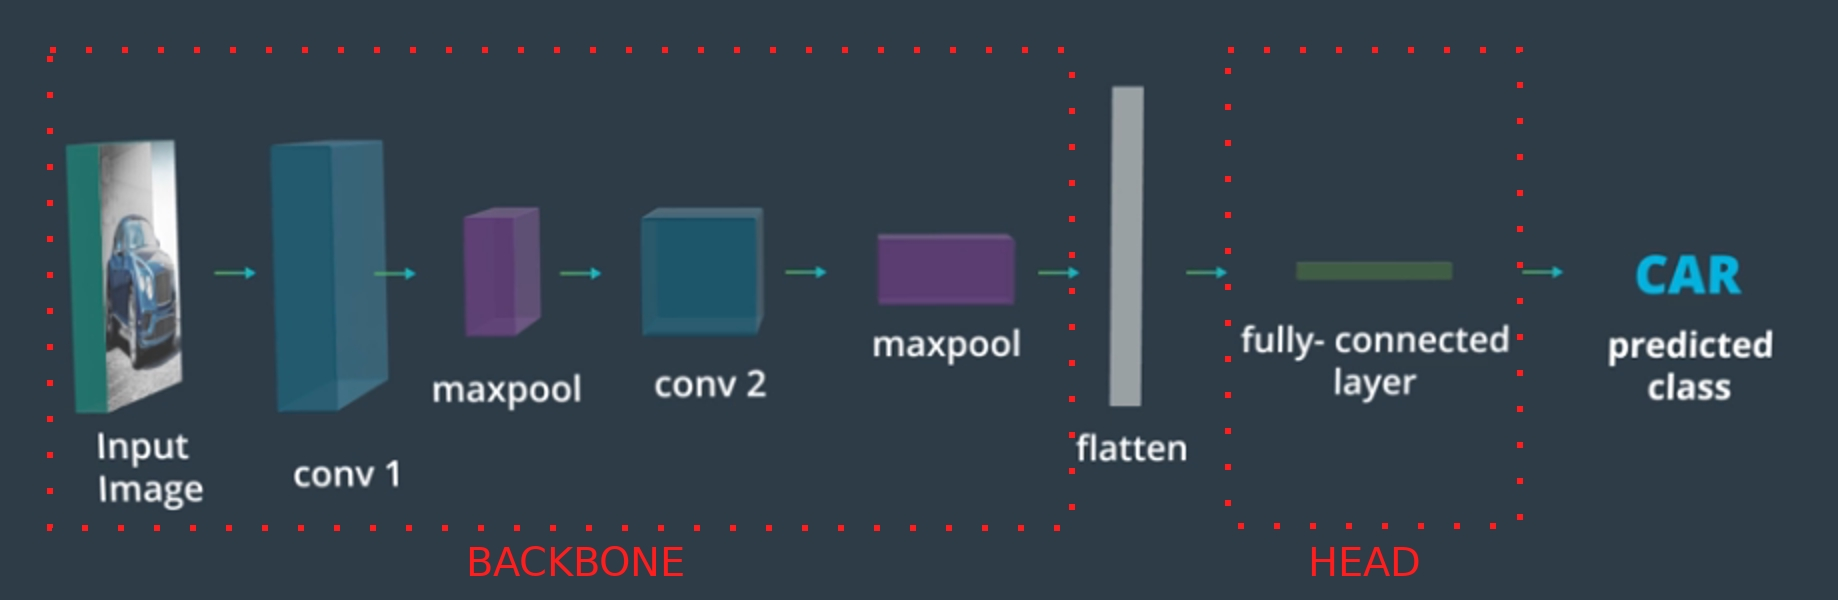
\includegraphics[width=1\linewidth]{img//cnn//depth/cnn-structure-complete.jpeg}

The \textbf{backbone} is made of convolutional and pooling layers, and has the task of extracting information from the image. \newline

After the backbone there is a flattening layer that takes the output feature maps of the previous convolutional layer and flattens them out in a 1d vector: for each feature map the rows are stacked together in a 1d vector, then all the 1d vectors are stacked together to form a long 1d vector called a \textbf{feature vector} or \textbf{embedding}. This process is illustrated by the following image:

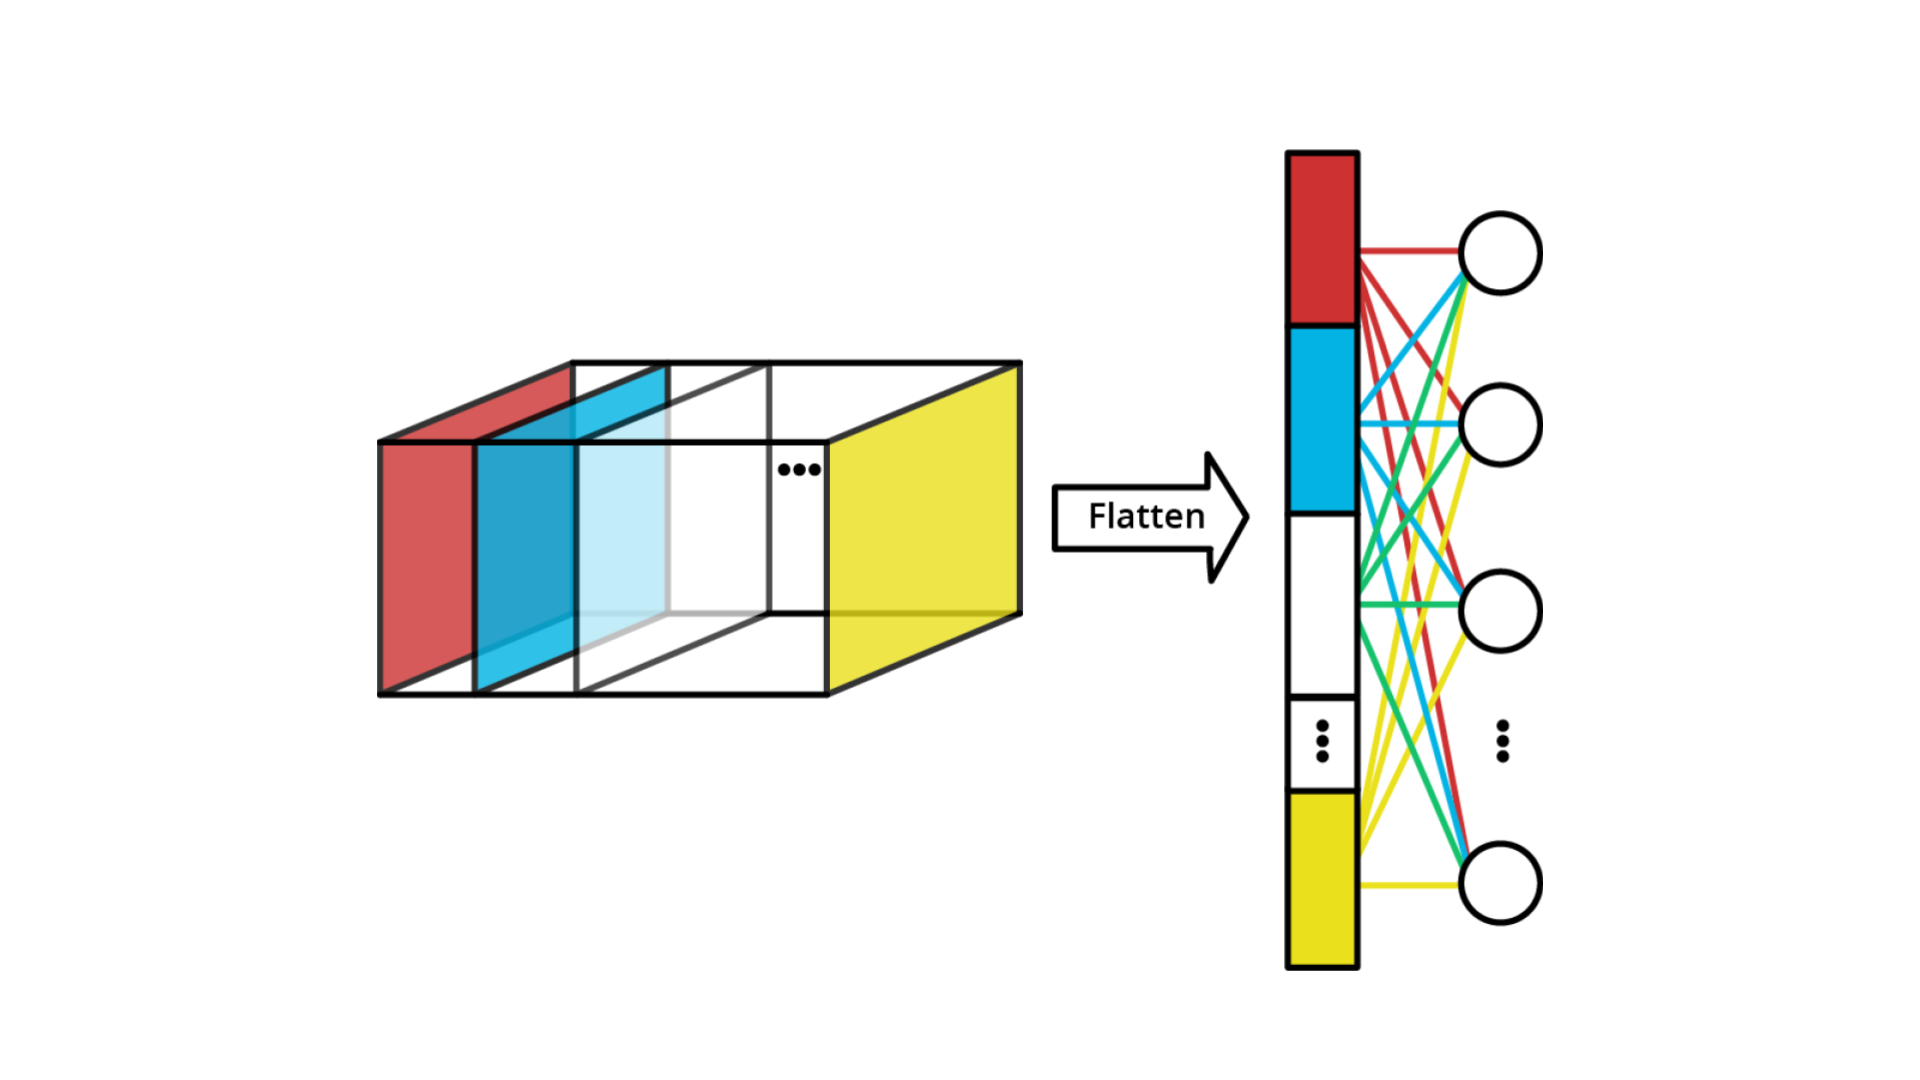
\includegraphics[width=0.75\linewidth]{img//cnn//depth/dlnd-refresh-c2-cd1821-l2-1.png}
\captionof{figure}{Feature Vector Process}

After the flattening operation we have the \textbf{head} section. The head is typically just a normal MLP that takes as input the feature vector and has the appropriate output for the task. It can have one or more hidden layers, as well as other types of layers as needed (like DropOut for regularization). In case of a classification task the output dimension is equal to the number of classes, just as in a normal MLP.


\section{CNNs in PyTorch: Summary So Far}

Now let's put everything together in code!

\subsection{The Typical Convolutional Block}

The typical sequence convolution -> pooling -> activation (with optional dropout) can be written in PyTorch like this:

\begin{lstlisting}
self.conv1 = nn.Conv2d(3, 16, 3, padding=1),
self.pool = nn.MaxPool2d(2, 2),
self.relu1 = nn.ReLU()
self.drop1 = nn.Dropout2d(0.2)
\end{lstlisting}
(or of course with the \lstinline{nn.Sequential} equivalent:
\begin{lstlisting}
self.conv_block = nn.Sequential(
  nn.Conv2d(3, 16, 3, padding=1),
  nn.MaxPool2d(2, 2),
  nn.ReLU(),
  nn.Dropout2d(0.2)
)
\end{lstlisting}
\subsection{A Simple CNN in PyTorch}

Let's now bring everything together and write our first CNN in PyTorch. We are going to have 3 convolutional blocks plus a head with a simple MLP.
\begin{lstlisting}
import torch
import torch.nn as nn

class MyCNN(nn.Module):

  def __init__(self, n_classes):

    super().__init__()

    # Create layers. In this case just a standard MLP
    self.model = nn.Sequential(
      # First conv + maxpool + relu
      nn.Conv2d(3, 16, 3, padding=1),
      nn.MaxPool2d(2, 2),
      nn.ReLU(),
      nn.Dropout2d(0.2),

      # Second conv + maxpool + relu
      nn.Conv2d(16, 32, 3, padding=1),
      nn.MaxPool2d(2, 2),
      nn.ReLU(),
      nn.Dropout2d(0.2),

      # Third conv + maxpool + relu
      nn.Conv2d(32, 64, 3, padding=1),
      nn.MaxPool2d(2, 2),
      nn.ReLU(),
      nn.Dropout2d(0.2),

      # Flatten feature maps
      nn.Flatten(),

      # Fully connected layers. This assumes
      # that the input image was 32x32
      nn.Linear(1024, 128),
      nn.ReLU(),
      nn.Dropout(0.5),
      nn.Linear(128, n_classes)
    )

  def forward(self, x):

    # nn.Sequential will call the layers 
    # in the order they have been inserted
    return self.model(x)
\end{lstlisting}
Let's analyze what is going on in the Sequential call. We have a series of 3 convolutional parts constituted of a convolutional layer, a max pooling operation that halves the input shape, and then a ReLU activation:
\begin{lstlisting}
nn.Conv2d(3, 16, 3, padding=1),
nn.MaxPool2d(2, 2),
nn.ReLU()
\end{lstlisting}
We can also optionally insert a \lstinline{nn.Dropout2d} layer for regularization. \newline

We repeat this structure 3 times, varying the number of feature maps in the sequence 16 -> 32 -> 64. As we go deep, in other words, we are working with feature maps with a smaller height and width (because we keep applying max pooling) but with a higher channel count. This is very typical and helps the network with abstracting concepts.\newline

Then, we have a \lstinline{Flatten} layer that flattens our 64 feature maps (coming from the last conv layer before the flattening) into one long vector. Assuming that the input is \(32 \times 32\), this vector will contain 1024 (\(4 \times 4 \times 64\)) numbers.\newline

Finally, we have an MLP made of fully-connected layers that combines all the information extracted by the convolutional part and outputs one number for each class (logits). We first compress the 1024-long array into an embedding of 128 numbers, and then from there to the number of classes we have.\newline

Since we have used the \lstinline{nn.Sequential} class, the \lstinline{forward} method is extremely simple and it is just calling that \lstinline{Sequential} instance.

\subsection{Quiz Question}

Consider the following network:
\begin{lstlisting}
from torch import  nn

model = nn.Sequential(
    nn.Conv2d(3, 16, kernel_size=3, padding=1),  # 224, 224
    nn.MaxPool2d(2, 2), # 112, 112
    nn.ReLU(),
    
    nn.Conv2d(16, 32, kernel_size=3, padding=0), # 110 x 110
    nn.MaxPool2d(2, 2),  # 55 x 55
    nn.ReLU()
)
\end{lstlisting}
Let's consider an image that is (3, 224, 224), i.e., an RGB image (3 channels) with height and width both equal to 224. If we push it through the network, what is the shape of the output?

HINT: The shape tuple is (n\_channels, height, width), where n\_channels is the number of output channels in the last layer.

\begin{itemize}
    \item (32, 56, 56)
    \item (32, 54, 54)
    \item \textbf{(32, 55, 55)}

\end{itemize}
Solutions: 
\begin{lstlisting}
nn.Conv2d(3, 16, kernel_size=3, padding=1),  # out shape: (16, 224, 224)
nn.MaxPool2d(2, 2), # (16, 112, 112)
nn.ReLU(),  # (16, 112, 112)
    
nn.Conv2d(16, 32, kernel_size=3, padding=0), # (32, 110, 110) [note that padding=0]
nn.MaxPool2d(2, 2),  # (32, 55, 55)
nn.ReLU() # (32, 55, 55)
\end{lstlisting}

\subsection{Quiz Question}

Consider the following network:
\begin{lstlisting}
model = nn.Sequential(
    nn.Conv2d(3, 16, kernel_size=3, padding=1),  # 224, 224
    nn.MaxPool2d(2, 2), # 112, 112
    nn.ReLU(),
    
    nn.Conv2d(16, 32, kernel_size=3, padding=0), # 110 x 110
    nn.MaxPool2d(2, 2),  # 55 x 55
    nn.ReLU(),
    
    nn.Flatten()
)
\end{lstlisting}
Let's consider an image that is (3, 224, 224), i.e., an RGB image (3 channels) with height and width both equal to 224. If we push it through the network, what is the shape of the output?
\begin{itemize}
    \item (32, 55, 55)
    \item \textbf{96800}
    \item 3025
\end{itemize}
Solution: Correct! 32 x 55 x 55 = 96800
\subsection{Quiz Question}

Consider the following CNN:
\begin{lstlisting}
model = nn.Sequential(
    nn.Conv2d(3, 16, kernel_size=3, padding=1),  # 224, 224
    nn.MaxPool2d(2, 2), # 112, 112
    nn.ReLU(),
    
    nn.Conv2d(16, 32, kernel_size=3, padding=0), # 110 x 110
    nn.MaxPool2d(2, 2),  # 55 x 55
    nn.ReLU(),
    
    nn.Flatten(),
    
    nn.Linear(feature_vector_dim, 512),
    nn.ReLU(),
    nn.Linear(512, 256),
    nn.ReLU(),
    nn.Linear(256, 100)
)
\end{lstlisting}
What should be the value of \lstinline{feature_vector_dim} in the first linear layer? In other words, what is the dimension of the feature vector that is fed to the head?

Also, how many classes does this classifier handle?
\begin{itemize}
    \item \textbf{feature\_vector\_dim = 96800, n\_classes = 100}
    \item feature\_vector\_dim = 96800, n\_classes = 256
    \item feature\_vector\_dim = (32, 55, 55), n\_classes = 256
    \item feature\_vector\_dim = (32, 55, 55), n\_classes = 100
\end{itemize}

\subsection{Quiz Question}

Consider this CNN (note that is slightly different than the previous ones!):
\begin{lstlisting}
model = nn.Sequential(
    nn.Conv2d(3, 16, kernel_size=3, padding=1), 
    nn.MaxPool2d(2, 2),
    nn.ReLU(),
    
    nn.Conv2d(16, 32, kernel_size=3, padding=1),
    nn.MaxPool2d(2, 2),
    nn.ReLU(),
    
    nn.Flatten(),
    
    nn.Linear(1568, 512),
    nn.ReLU(),
    nn.Linear(512, 256),
    nn.ReLU(),
    nn.Linear(256, 100)
)
\end{lstlisting}
Please check all the true sentences:
\begin{itemize}
    \item \textbf{There are 2 convolutional layers plus an MLP with one hidden layer, one input layer, and one output layer.}
    \item This network can handle images that are 224 by 224 in size.
    \item \textbf{This network can handle images that are 28 by 28 in size.}
    \item \textbf{There are 100 classes.}
\end{itemize}

\section{Solution: CNNs for CIFAR Image Classification}
\begin{itemize}
    \item \href{https://www.youtube.com/watch?v=N6XMFPmXysk&t=1s&ab_channel=Udacity}{Load data}
    \item \href{https://www.youtube.com/watch?v=4XaDhzZsx9c&t=70s&ab_channel=Udacity}{Create architecture}
    \item \href{https://www.youtube.com/watch?v=Aw0D_u5-7wc&ab_channel=Udacity}{Train and test the network}
\end{itemize}

\section{Image Augmentation}

\subsection{Optimizing the Performance of Our Network}

Now that we have seen how to train a simple CNN, let’s dive deeper and see how we can improve on the performance of our network with some widely-adopted tricks.\newline

The first one is \textbf{image augmentation}. \href{https://www.youtube.com/watch?v=OEzHz9USHWY&t=2s&ab_channel=Udacity}{Youtube}

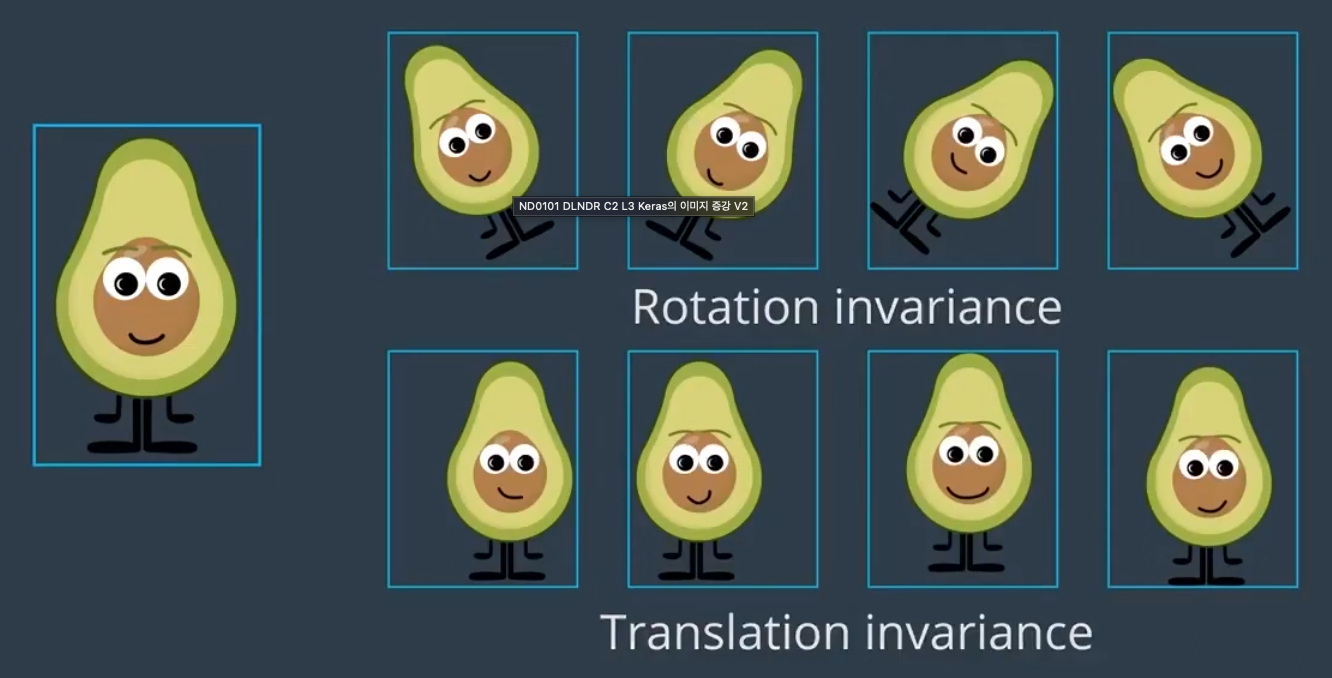
\includegraphics[width=1\linewidth]{img//cnn//depth/imageaugmentation.png}

The basic idea of image augmentation is the following: if you want your network to be insensitive to changes such as rotation, translation, and dilation, you can use the same input image and rotate it, translate it, and scale it and ask the network not to change its prediction! \newline

In practice, this is achieved by applying random transformations to the input images before they are fed to the network.

\section{Augmentation Using Transformations}
\href{https://www.youtube.com/watch?v=RUNIokjb2vM&ab_channel=Udacity}{Youtube} \newline

Image augmentation is a very common method to:

\begin{enumerate}
    \item Increase the robustness of the network
    \item Avoid overfitting
    \item Introduce rotational, translational and scale invariance as well as insensitiveness to color changes
    \item Avoid \href{https://news.mit.edu/2021/shortcut-artificial-intelligence-1102}{\textbf{shortcut learning}}
\end{enumerate}

\subsection{Demo: Augmentation Using Transformations}
\href{https://www.youtube.com/watch?v=HxhC6rs72cs&ab_channel=Udacity}{Youtube} \newline

\subsection{Augmentation Pipelines}

A typical training augmentation pipeline is represented in this diagram.

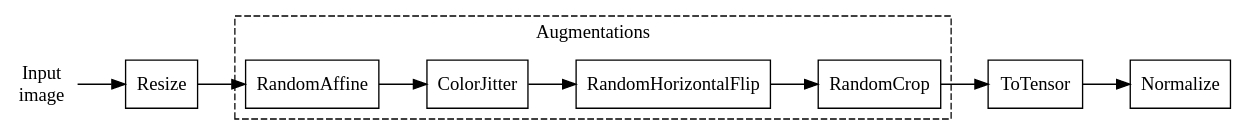
\includegraphics[width=1\linewidth]{img//cnn//depth/train-aug1.jpeg}
\captionof{figure}{Typical Training Augmentation Pipeline}

This typical training augmentation pipeline can be implemented in PyTorch as follows (transforms are documented \href{https://pytorch.org/vision/main/transforms.html}{\textbf{here}}):

\begin{lstlisting}
import torchvision.transforms as T


train_transforms = T.Compose(
    [
        # The size here depends on your application. Here let's use 256x256
        T.Resize(256),
        # Let's apply random affine transformations (rotation, translation, shear)
        # (don't overdo here!)
        T.RandomAffine(scale=(0.9, 1.1), translate=(0.1, 0.1), degrees=10),
        # Color modifications. Here I exaggerate to show the effect 
        T.ColorJitter(brightness=0.5, contrast=0.5, saturation=0.5, hue=0.5),
        # Apply an horizontal flip with 50% probability (i.e., if you pass
        # 100 images through around half of them will undergo the flipping)
        T.RandomHorizontalFlip(0.5),
        # Finally take a 224x224 random part of the image
        T.RandomCrop(224, padding_mode="reflect", pad_if_needed=True),  # -
        T.ToTensor(),
        T.Normalize((0.5, 0.5, 0.5), (0.5, 0.5, 0.5)),
    ]
)
\end{lstlisting}

This pipeline produces variations of the same image as this example:

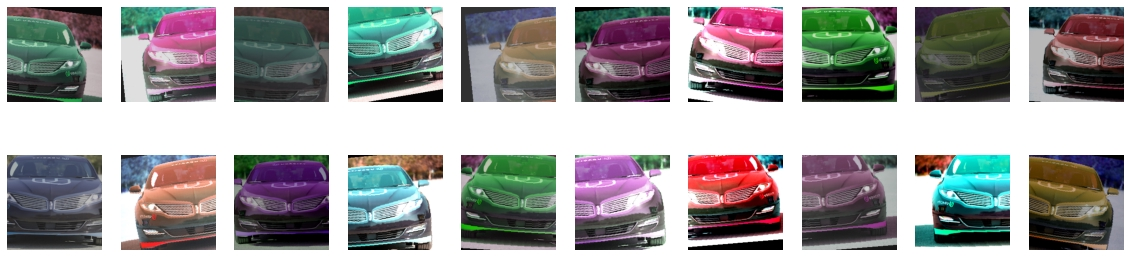
\includegraphics[width=1\linewidth]{img//cnn//depth/augmentations.jpeg}
\captionof{figure}{Image Augmentations}

\href{https://www.youtube.com/watch?v=SeStXrarAtQ&ab_channel=Udacity}{Youtube}

\subsection{Transformation Pipelines for Validation and Test}

During validation and test you typically do not want to apply image augmentation (which is needed for training). Hence, this is a typical transform pipeline for validation and test that can be paired with the pipeline above:
\begin{lstlisting}
testval_transforms = T.Compose(
    [
        # The size here depends on your application. Here let's use 256x256
        T.Resize(256),
        # Let's take the central 224x224 part of the image
        T.CenterCrop(224),
        T.ToTensor(),
        T.Normalize((0.5, 0.5, 0.5), (0.5, 0.5, 0.5)),
    ]
)
\end{lstlisting}
Note that of course:

\begin{itemize}
    \item The resize and crop should be the same as applied during training for best performance
    \item The normalization should be the same between training and inference (validation and test)
\end{itemize}

\subsection{AutoAugment Transforms}

There is a special class of transforms defined in \lstinline{torchvision}, referred to as \href{https://pytorch.org/vision/main/transforms.html\#automatic-augmentation-transforms}{\textbf{AutoAugment}}. These classes implements augmentation policies that have been optimized in a data-driven way, by performing large-scale experiments on datasets such as ImageNet and testing many different recipes, to find the augmentation policy giving the best result. It is then proven that these policies provide good performances also on datasets different from what they were designed for. \newline

For example, one such auto-transform is called \lstinline{RandAugment} and it is widely used. It is particularly interesting because it parametrizes the strength of the augmentations with one single parameter that can be varied to easily find the amount of augmentations that provides the best results. This is how to use it:
\begin{lstlisting}
T.RandAugment(num_ops, magnitude)
\end{lstlisting}
The main parameters are:

\begin{itemize}
    \item \lstinline{num_ops}: the number of random transformations applied. Defaut: 2
    \item \lstinline{magnitude}: the strength of the augmentations. The larger the value, the more diverse and extreme the augmentations will become.
\end{itemize}
As usual, refer to the \href{https://pytorch.org/vision/main/generated/torchvision.transforms.RandAugment.html\#torchvision.transforms.RandAugment}{\textbf{official documentation}} for details.

\section{Batch Normalization}

The second modern trick that paves the way for enhancing the performance of a network is called \textbf{Batch Normalization,} or \textbf{BatchNorm}. It does not usually improve the performances per se, but it allows for much easier training and a much smaller dependence on the network initialization, so in practice it makes our experimentation much easier, and allows us to more easily find the optimal solution. \newline

\href{https://www.youtube.com/watch?v=Ot2ObfYuGKk&t=3s&ab_channel=Udacity}{Youtube}

\subsection{How BatchNorm Works}

Just as we normalize the input image before feeding it to the network, we would like to keep the feature maps normalized, since they are the output of one layer and the input to the next layer. In particular, we want to prevent them to vary wildly during training, because this would require large adjustments of the subsequent layers. Enter BatchNorm. BatchNorm normalizes the activations and keep them much more stable during training, making the training more stable and the convergence faster. \[x \leftarrow \frac{x - \mu_x}{\sigma_x} \gamma + \beta\]
where 
\begin{itemize}
    \item \(x\): activations (for exmaple, values in the feature maps)
    \item \(\mu_x\): mean of the activations
    \item \(\sigma_x\) standard deviation of the activations
    \item \(\gamma\) and \(\beta\): learnable parameters
\end{itemize}

In order to do this, during training BatchNorm needs the mean and the variance for the activations for each mini-batch. This means that the batch size cannot be too small or the estimates for mean and variance will be inaccurate. During training, the BatchNorm layer also keeps a running average of the mean and the variance, to be used during inference. \newline

During inference we don't have mini-batches. Therefore, the layer uses the mean and the variance computed during training (the running averages). \newline

This means that BatchNorm behaves differently during training and during inference. The behavior changes when we set the model to training mode (using \lstinline{model.train()}) or to validation mode (\lstinline{model.eval()}).

\subsection{Pros and Cons of Batch Normalization}
\href{https://www.youtube.com/watch?v=75KLWEruuLs&t=1s&ab_channel=Udacity}{Youtube} \newline

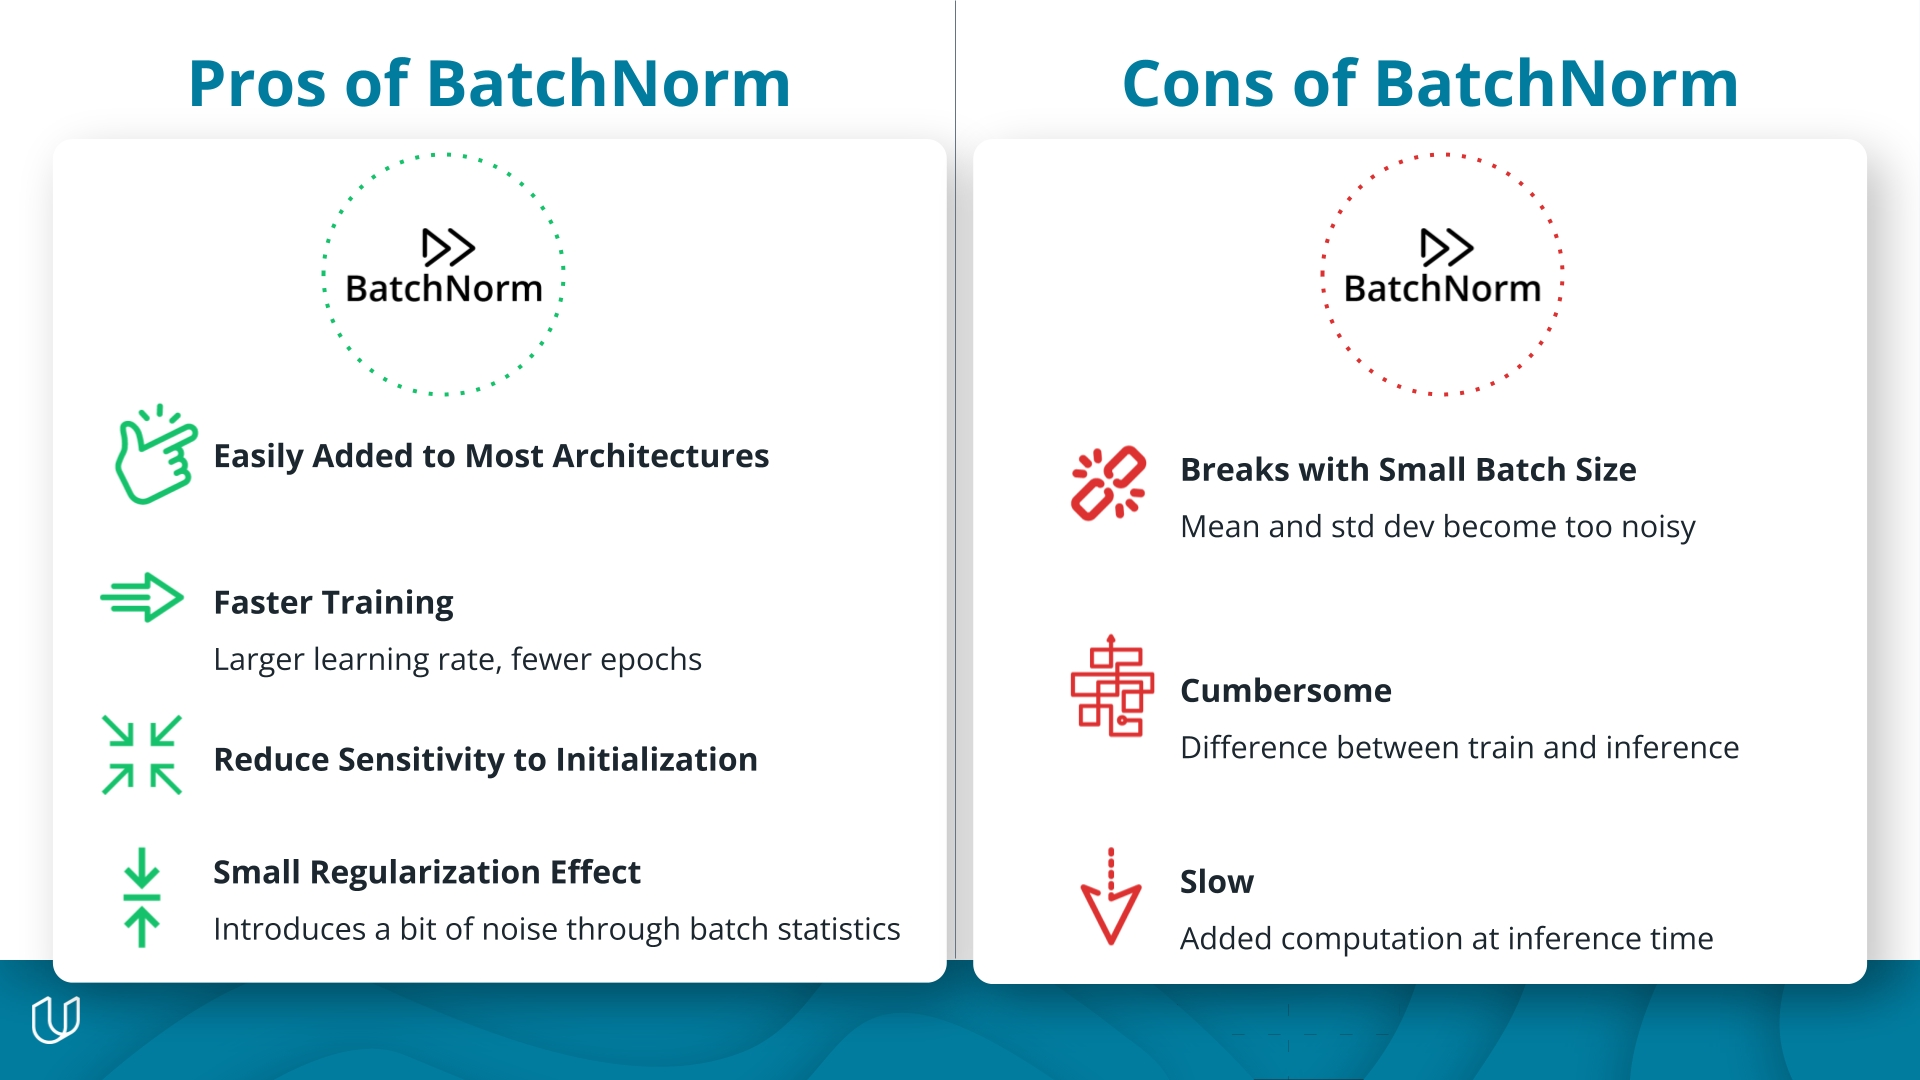
\includegraphics[width=1\linewidth]{img//cnn//depth/dlnd-refresh-c2-cd1821-cnns-l3.jpeg}

These advantages of using BatchNorm generally outweigh these disadvantages, so BatchNorm is widely used in almost all CNN implementations today.


\section{BatchNorm in PyTorch}
\href{https://www.youtube.com/watch?v=cvYC40wyo2U&t=1s&ab_channel=Udacity}{Youtube}. Notice on Youtube video: At 0:49, the instructor says to put \textbf{BachNorm} after \textbf{Dropout}, which is incorrect. \textbf{Dropout} drops some connections only at training time, so placing it before \textbf{BatchNorm} would cause the distribution seen by \textbf{BatchNorm} to be different between training and inference. Therefore, \textbf{BatchNorm} should be placed before \textbf{Dropout}.

\subsection{BatchNorm for Convolutional Layers}

BatchNorm can be used very easily in PyTorch as part of the convolutional block by adding the \lstinline|nn.BatchNorm2d| layer just after the convolution:
\begin{lstlisting}
self.conv1 = nn.Sequential(
  nn.Conv2d(3, 16, kernel_size=3, padding=1),
  nn.BatchNorm2d(16),
  nn.MaxPool2d(2, 2),
  nn.ReLU(),
  nn.Dropout2d(0.2)
)
\end{lstlisting}
The only parameter is the number of input feature maps, which of course must be equal to the output channels of the convolutional layer immediately before it.

\textit{NOTE}: It is important to use \lstinline|BatchNorm| before DropOut. The latter drops some connections only at training time, so placing it before \lstinline|BatchNorm| would cause the distribution seen by BatchNorm to be different between training and inference.

\subsection{BatchNorm for Dense Layers}

We can add BatchNorm to MLPs very easily by using \lstinline|nn.BatchNorm1d|:
\begin{lstlisting}
self.mlp = nn.Sequential(
  nn.Linear(1024, 500),
  nn.BatchNorm1d(500),
  nn.ReLU(),
  nn.Dropout(0.5)
)
\end{lstlisting}

\section{Optimizing the Performance of Our Network}
\href{https://www.youtube.com/watch?v=8YpN0GxOKmw&ab_channel=Udacity}{Youtube}

\subsection{Important Terms in Optimizing Performance}

\textbf{Parameter}
\begin{itemize}
    \item Internal to the model
    \item May vary during training
    \item Examples: Weights and biases of a network
\end{itemize}

\textbf{Hyperparameter}
\begin{itemize}
    \item External to the model
    \item Fixed during training
    \item Examples: Learning rate, number of layers, activation layers
\end{itemize}

\textbf{Experiment}
\begin{itemize}
    \item A specific training run with a fixed set of hyperparameters
    \item Practitioners typically perform many experiments varying the hyperparameters. Each experiment produces one or more metrics that can be used to select the best-performing set of hyperparameters (see the next section).
\end{itemize}

\subsection{Strategies for Optimizing Hyperparameters}

\begin{itemize}
    \item \textbf{Grid search}

\begin{itemize}
        \item Divide the parameter space in a regular grid
        \item Execute one experiment for each point in the grid
        \item Simple, but wasteful
\end{itemize}

    \item \textbf{Random search}

\begin{itemize}
        \item Divide the parameter space in a random grid
        \item Execute one experiment for each point in the grid
        \item Much more efficient sampling of the hyperparameter space with respect to grid search
\end{itemize}

    \item \textbf{Bayesian Optimization}

\begin{itemize}
        \item Algorithm for searching the hyperparameter space using a Gaussian Process model
        \item Efficiently samples the hyperparameter space using minimal experiments
\end{itemize}

\end{itemize}

\subsection{Most Important Hyperparameters}
\href{https://www.youtube.com/watch?v=QJi0ORH3k0E&ab_channel=Udacity}{Youtube}

\subsection{Summary: Most Important Hyperparameters}

Optimizing hyperparameters can be confusing at the beginning, so we provide you with some rules of thumb about the actions that typically matter the most. They are described in order of importance below. These are not strict rules, but should help you get started:

\begin{enumerate}
    \item Design parameters: When you are designing an architecture from scratch, the number of hidden layers, as well as the layers parameters (number of filters, width and so on) are going to be important.
    \item Learning rate: Once the architecture is fixed, this is typically the most important parameter to optimize. The next video will focus on this.
    \item Batch size: This is typically the most influential hyperparameter after the learning rate. A good starting point, especially if you are using BatchNorm, is to use the maximum batch size that fits in the GPU you are using. Then you vary that value and see if that improves the performances.
    \item Regularization: Once you optimized the learning rate and batch size, you can focus on the regularization, especially if you are seeing signs of overfitting or underfitting.
    \item Optimizers: Finally, you can also fiddle with the other parameters of the optimizers. Depending on the optimizers, these vary. Refer to the documentation and the relevant papers linked there to discover what these parameters are.
\end{enumerate}

\subsection{Optimizing Learning Rate}
\href{https://www.youtube.com/watch?v=nyFpT0Xj860&t=3s&ab_channel=Udacity}{Youtube}

\subsubsection{Summary: Optimizing Learning Rate}

The learning rate is one of the most important hyperparameters. However, knowing what the optimal value is, or even what a good range is, can be challenging. \newline

One useful tool to discover a good starting point for the learning rate is the so-called "learning rate finder." It scans different values of the learning rate, and computes the loss obtained by doing a forward pass of a mini-batch using that learning rate. Then, we can plot the loss vs. the learning rate and obtain a plot similar to this:

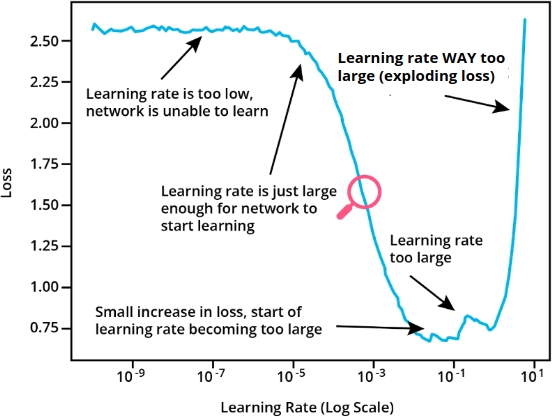
\includegraphics[width=0.5\linewidth]{img//cnn//depth/lr-finder.jpeg}

We want to pick as a starting point the learning rate corresponding to more or less the middle of the steep part of the graph (indicated by the red marker in the plot).

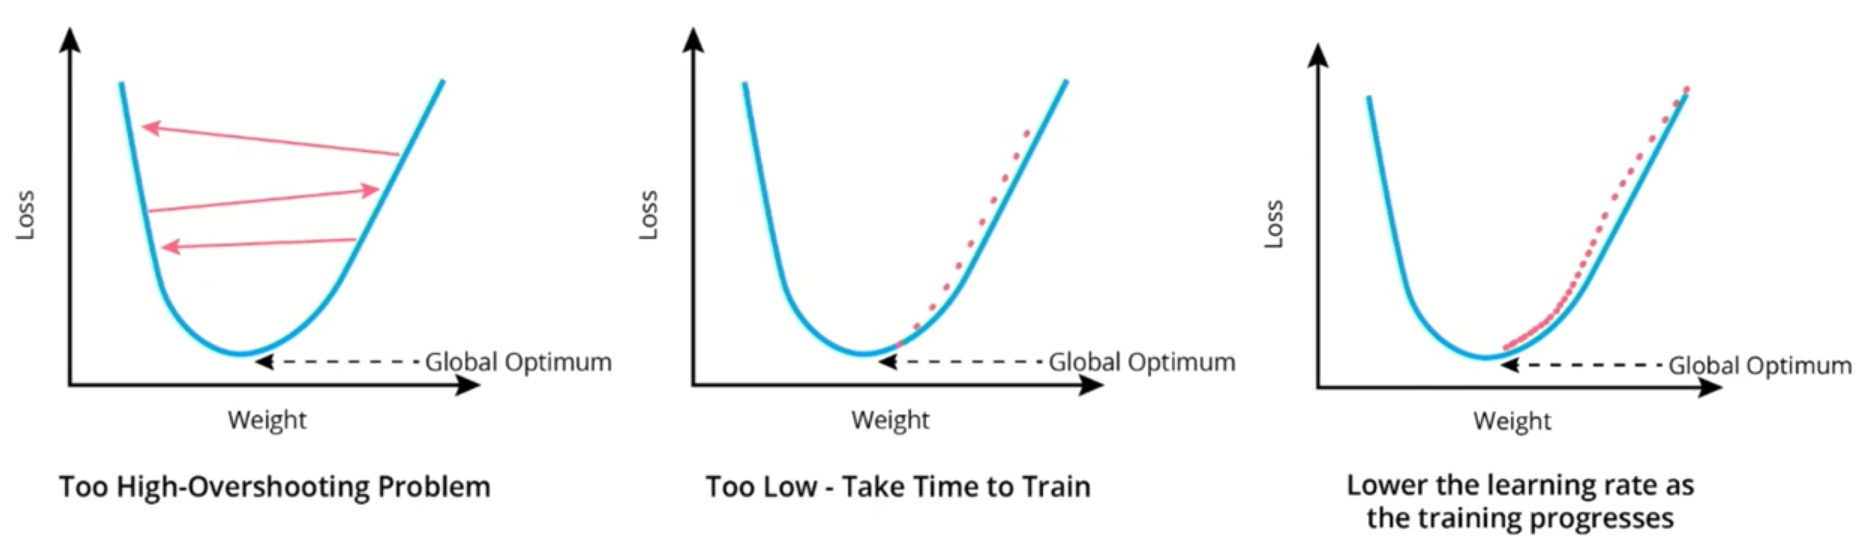
\includegraphics[width=1\linewidth]{img//cnn//depth/learningrateoptimization.png}

\subsubsection{Learning Rate Schedulers}

In many cases we want to vary the learning rate as the training progresses. At the beginning of the training we want to make pretty large steps because we are very far from the optimum. However, as we approach the minimum of the loss, we need to make sure we do not jump over the minimum. \newline

For this reason, it is often a good idea to use a \textbf{learning rate scheduler}, i.e., a class that changes the learning rate as the training progresses. \newline

There are several possible learning rate schedulers. You can find the available ones in the \href{https://pytorch.org/docs/stable/optim.html\#how-to-adjust-learning-rate}{\textbf{documentation}}. \newline

One of the simplest one is the \lstinline{StepLR} scheduler. It reduces the learning rate by a specific factor every \lstinline{n} epochs. It can be used as follows:
\begin{lstlisting}
from torch.optim.lr_scheduler import StepLR

scheduler = StepLR(optimizer, step_size=5, gamma=0.5)

# Training loop
for ... 
    ...
    # Update the weights
    optimizer.step()

    # Update the learning rate in the
    # optimizer according to the schedule
    scheduler.step()
\end{lstlisting}
\section{Tracking Your Experiments}

\subsection{Tracking Your Experiments}

When you are performing hyperparameter optimization and other changes it is very important that you track all of your experiments. This way you will know which hyperparameters have given you which results, and you will be able to repeat those experiments, choose the best one, understand what works and what doesn't, and what you need to explore further. You will also be able to present all your results to other people.\newline

You can of course use spreadsheets for this, or even pen and paper, but there are definitely much better ways!\newline

Enter experiment tracking tools. There are many of them out there, and they all work in similar ways. Let's consider \href{https://www.mlflow.org/docs/latest/tracking.html}{\textbf{mlflow}}, which is free and open source.\newline

Tracking an experiment is easy in mlflow. You first start by creating a run. A run is a unit of execution that will contain your results. Think of it as one row in a hypothetical spreadsheet, where the columns are the things you want to track (accuracy, validation loss, ...). A run can be created like this:
\begin{lstlisting}
with mlflow.start_run():
  ... your code here ...
\end{lstlisting}
Once you have created the run, you can use \lstinline{mlflow.log_param} to log a parameter (i.e., one of the hyperparameters for example) and \lstinline{mlflow.log_metric} to log a result (for example the final accuracy of your model). For example, let's assume that our only hyperparameters are the learning rate and the batch size. We can track their values as well as the results obtained when using those values like this:
\begin{lstlisting}
import mlflow

with mlflow.start_run():

        ... train and validate ...

    # Track values for hyperparameters    
    mlflow.log_param("learning_rate", learning_rate)
    mlflow.log_param("batch_size", batch_size)

    # Track results obtained with those values
    mlflow.log_metric("val_loss", val_loss)
    mlflow.log_metric("val_accuracy", val_accuracy)

    # Track artifacts (i.e. files produced by our experiment)
    # For example, we can save the weights for the epoch with the
    # lowest validation loss
    mlflow.log_artifact("best_valid.pt")
\end{lstlisting}
If we do this for all of our experiments, then \lstinline|mlflow| will allow us to easily study the results and understand what works and what doesn't. It provides a UI that looks like this:

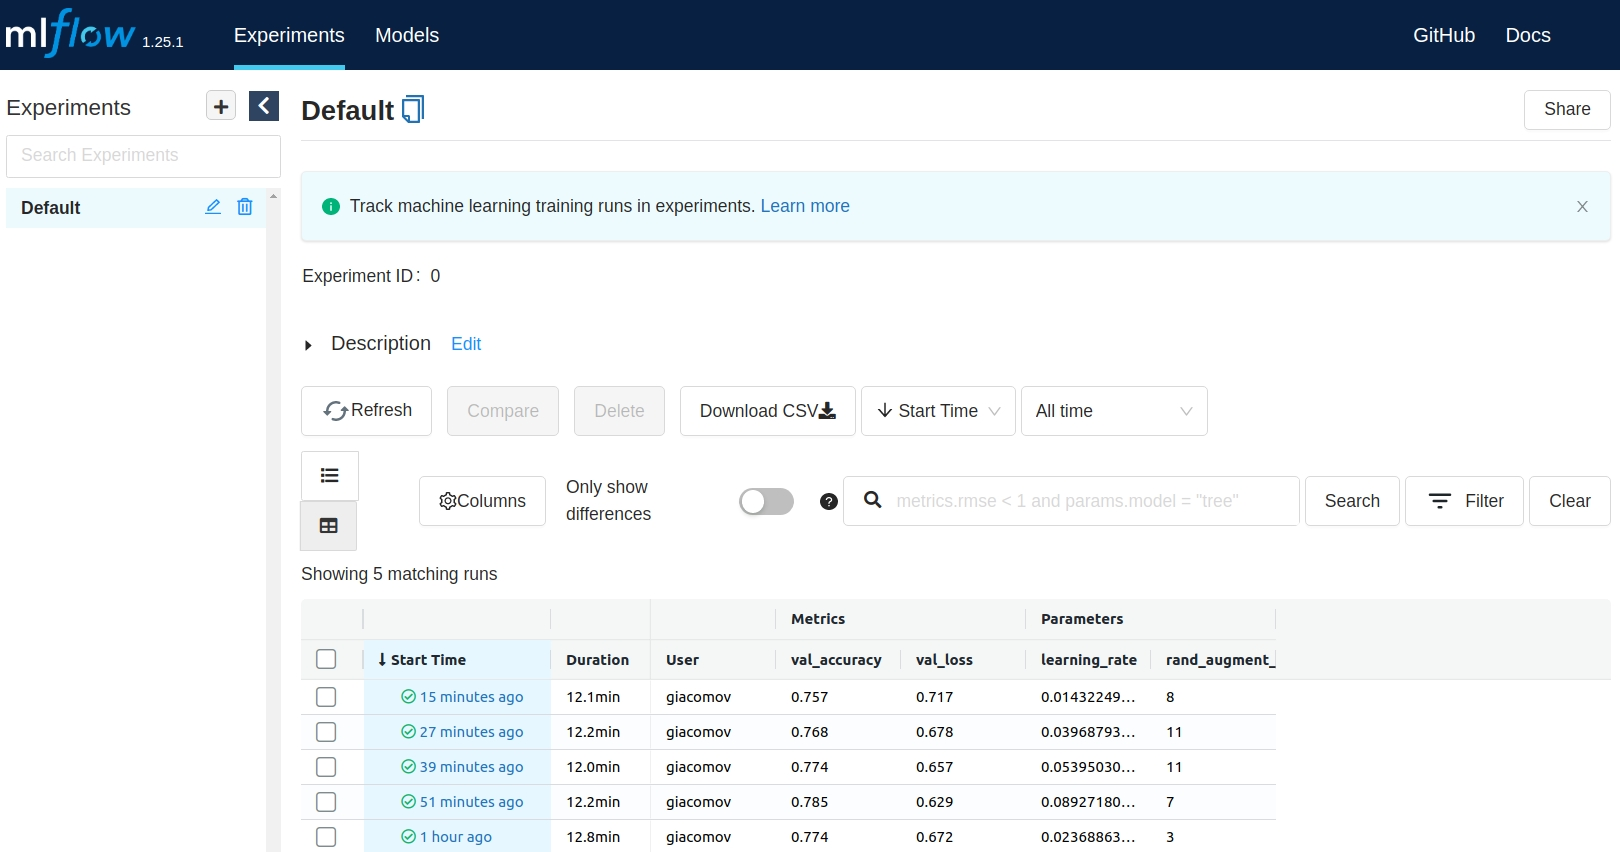
\includegraphics[width=1\linewidth]{img//cnn//depth/mlflow.jpeg}
\captionof{figure}{The mlflow Experiment-Tracking UI}

But you can also look at the results in a notebook by doing:
\begin{lstlisting}
runs = mlflow.search_runs()
\end{lstlisting}
\lstinline{runs} is a pandas DataFrame that you can use to look at your results. \newline

We barely scratched the surface about what a tracking tool like \lstinline{mlflow} can do for you. For example, they track the code that runs in your experiment so you can reproduce it even if you changed the code in the meantime. If you are looking to apply what you are learning in this course in a professional environment, have a good look at tracking tools and how they can benefit you.

\section{Quiz Question}

What are some techniques to improve the performance of a CNN? (may be more than one answer)
\begin{itemize}
    \item \textbf{Image augmentations}
    \item \textbf{Hyperparameter tuning}
    \item Tracking your experiments
    \item Use larger networks
    \item Train for longer
    \item \textbf{Use a learning rate scheduler}
\end{itemize}

\section{Quiz Question}

What is the role of the BatchNorm layer in modern CNNs? Select all that apply.
\begin{itemize}
    \item \textbf{Standardize the activations of a layer to prevent covariate shift (i.e., shifts in the distribution of the activations)}
    \item Decrease the input size by 2
    \item \textbf{Allow for faster training and larger learning rates}
    \item \textbf{Makes the layers more independent from each other, making the work of the optimizer much easier}
    \item Improve the accuracy of the network
\end{itemize}

\section{Quiz Question}
Use this output from the learning rate finder for the next quiz question:

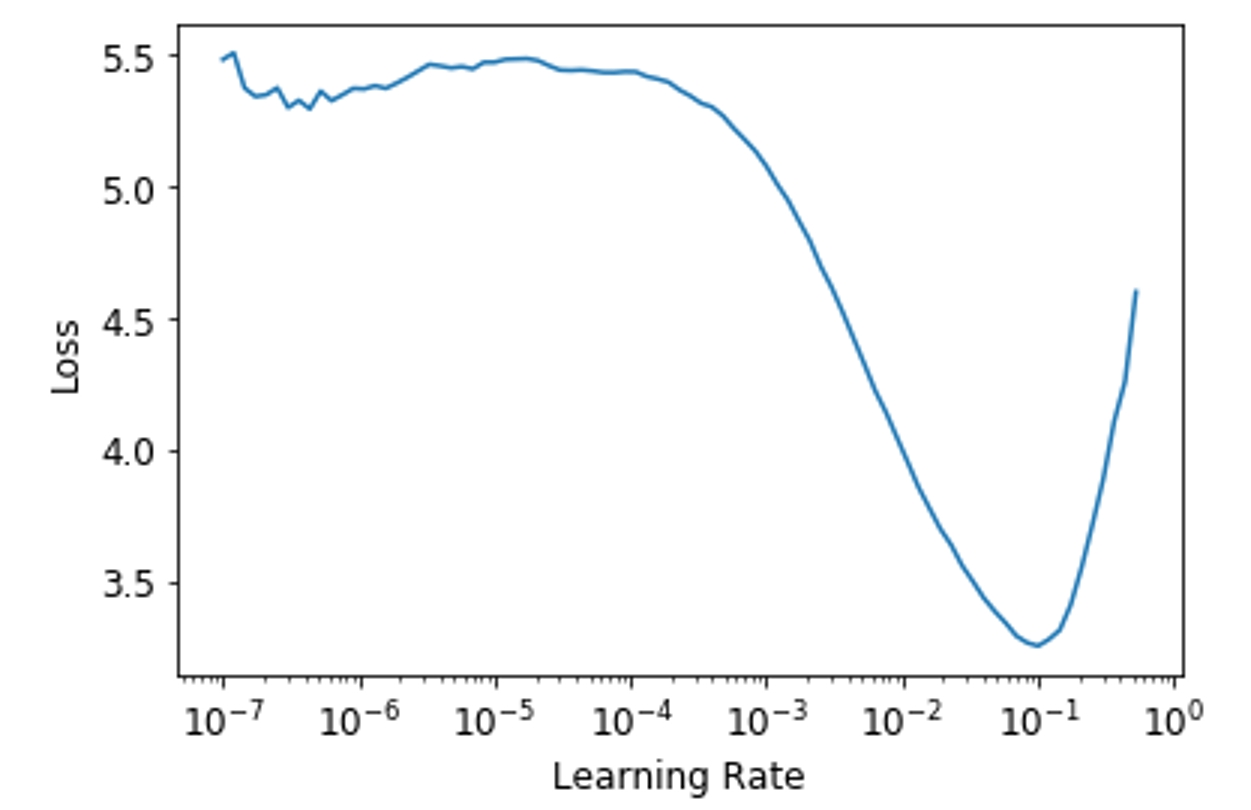
\includegraphics[width=1\linewidth]{img//cnn//depth/lr-finderjty.jpeg}

Which one is a sensible choice for the learning rate:
\begin{itemize}
    \item 0.1
    \item 0.00001 (1e-5)
    \item \textbf{0.005 (5e-3)}
\end{itemize}

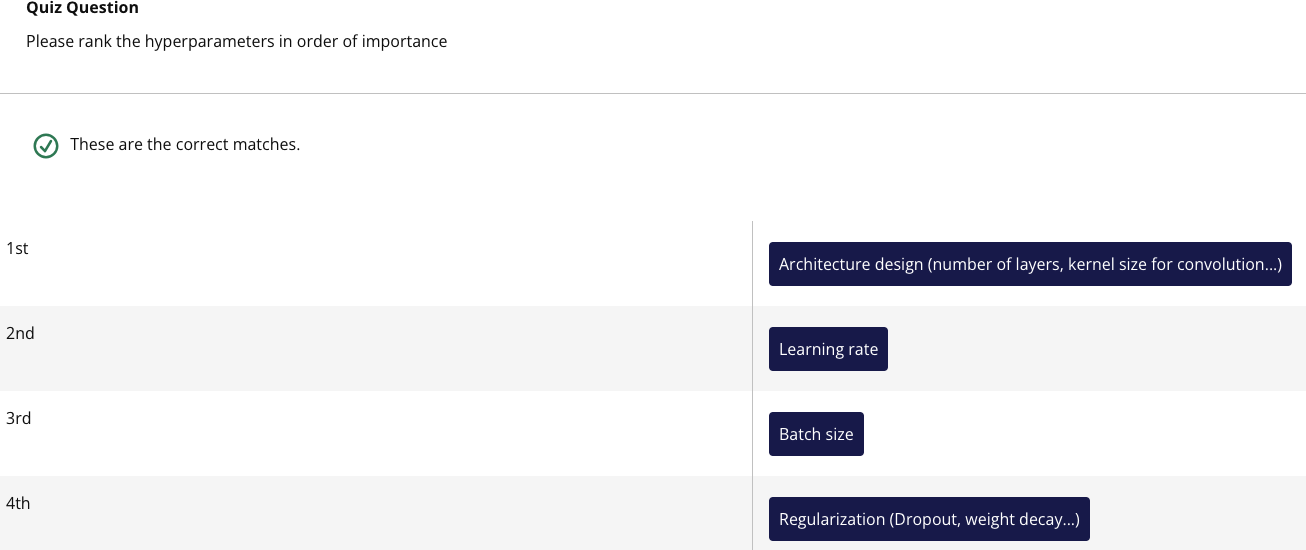
\includegraphics[width=1\linewidth]{img//cnn//depth/imagequiz.png}


\section{Exercise Solution: Improving Performance}
\begin{itemize}
    \item \href{https://www.youtube.com/watch?v=azxWs3Q9PN0&t=42s&ab_channel=Udacity}{Solution, Part 1: Data Augmentation, Model Definition}
    \item \href{https://www.youtube.com/watch?v=HWC4Rp0d29g&ab_channel=Udacity}{Solution, Part 2: Running and Tracking Experiments to Optimize Hyperparameters}
\end{itemize}


\section{Weight Initialization}

\subsection{What is Weight Initialization?}

Weight initialization is a procedure that happens only once, before we start training our neural network. Stochastic Gradient Descent and other similar algorithms for minimization are iterative in nature. They start from some values for the parameters that are being optimized and they change those parameters to achieve the minimum in the objective function (the loss).\newline

These "initial values" for the parameters are set through \textbf{weight initialization}.\newline

Before the introduction of BatchNorm, weight initialization was really key to obtaining robust performances. In this previous era, a good weight initialization strategy could make the difference between an outstanding model and one that could not train at all. These days networks are much more forgiving. However, a good weight initialization can speed up your training and also give you a bit of additional performance.\newline

In general, weights are initialized with random numbers close but not equal to zero, not too big but not too small either. This makes the gradient of the weights in the initial phases of training neither too big nor too small, which promotes fast training and good performances. Failing to initialize the weights well could result in \href{https://en.wikipedia.org/wiki/Vanishing_gradient_problem}{\textbf{vanishing or exploding gradients}}, and the training would slow down or stop altogether.

\subsection{Weight Initialization in PyTorch}

By default, PyTorch uses specific weight initialization schemes for each type of layer. This in practice means that you rarely have to think about weight initialization, as the framework does it for you using high-performance default choices.\newline

If you are curious, you can see how each layer is initialized by looking at the \lstinline{reset_parameters} method in the code for that layer. For example, \href{https://github.com/pytorch/pytorch/blob/f9d07ae6449224bdcb6eb69044a33f0fb5780adf/torch/nn/modules/linear.py\#L92}{\textbf{this is the initialization strategy for a Linear layer}} (i.e., a fully-connected layer), and \href{https://github.com/pytorch/pytorch/blob/f9d07ae6449224bdcb6eb69044a33f0fb5780adf/torch/nn/modules/conv.py\#L140}{\textbf{this is the initialization strategy for a Conv2d layer}}. In both cases PyTorch uses the so-called \href{https://paperswithcode.com/method/he-initialization}{\textbf{He initialization}} (or Kaiming initialization).

\section{Export a Model for Production}

\subsection{Wrap Your Model for Inference}

Exporting a model for production means packaging your model in a stand-alone format that can be transferred and used to perform inference in a production environment, such as an API or a website.

\subsubsection{Production-Ready Preprocessing}

Remember that the images need some preprocessing before being fed to the CNN. For example, typically you need to resize, center crop, and normalize the image with a transform pipeline similar to this:
\begin{lstlisting}
testval_transforms = T.Compose(
    [
        # The size here depends on your application. Here let's use 256x256
        T.Resize(256),
        # Let's take the central 224x224 part of the image
        T.CenterCrop(224),
        T.ToTensor(),
        T.Normalize((0.5, 0.5, 0.5), (0.5, 0.5, 0.5)),
    ]
)
\end{lstlisting}

Obviously, if you do not do these operations in production the performance of your model is going to suffer greatly. \newline

The best course of action is to make these transformations part of your standalone package instead of re-implementing them in the production environment. Let's see how.\newline

We need to wrap our model in a wrapper class that is going to take care of applying the transformations and then run the transformed image through the CNN.

If we trained with the \lstinline{nn.CrossEntropyLoss} as the loss function, we also need to apply a softmax function to the output of the model so that the output of the wrapper will be probabilities and not merely scores.\newline

Let's see an example of such a wrapper class:
\begin{lstlisting}
import torch
from torchvision import datasets
import torchvision.transforms as T
from __future__ import annotations


class Predictor(nn.Module):

    def __init__(
      self, 
      model: nn.Module, 
      class_names: list[str], 
      mean: torch.Tensor, 
      std: torch.Tensor
    ):

        super().__init__()

        self.model = model.eval()
        self.class_names = class_names

        self.transforms = nn.Sequential(
            T.Resize([256, ]),
            T.CenterCrop(224),
            T.ConvertImageDtype(torch.float),
            T.Normalize(mean.tolist(), std.tolist())
        )

    def forward(self, x: torch.Tensor) -> torch.Tensor:
        with torch.no_grad():
            # 1. apply transforms
            x = self.transforms(x)  # =
            # 2. get the logits
            x = self.model(x)  # =
            # 3. apply softmax
            #    HINT: remmeber to apply softmax across dim=1
            x = F.softmax(x, dim=1)  # =

            return x
\end{lstlisting}

\subsubsection{The Constructor}

Let's first look at the constructor \lstinline{__init__}: we first set the model to eval mode, and we also save the class names. This will be useful in production: the wrapper will return the probability for each class, so if we take the maximum of that probability and take the corresponding element from the \lstinline{class_names} list, we can return the winning label.

Then we have this:
\begin{lstlisting}
self.transforms = nn.Sequential(
            T.Resize([256, ]),  # We use single int value inside a list due to torchscript type restrictions
            T.CenterCrop(224),
            T.ConvertImageDtype(torch.float),
            T.Normalize(mean.tolist(), std.tolist())
        )
\end{lstlisting}

This defines the transformations we want to apply. It looks very similar to the transform validation pipeline, with a few important differences:

\begin{itemize}
    \item We do not use \lstinline{nn.Compose} but \lstinline{nn.Sequential}. Indeed the former is not supported by \lstinline{torch.script} (the export functionality of PyTorch).
    \item In \lstinline{Resize} the size specification must be a tuple or a list, and not a scalar as we were able to do during training.
    \item There is no \lstinline{ToTensor}. Instead, we use \lstinline{T.ConvertImageDtype}. Indeed, in this context the input to the forward method is going to be already a Tensor
\end{itemize}

\subsubsection{The \lstinline{forward} Method}

Let's now look at the \lstinline{forward} method:
\begin{lstlisting}
def forward(self, x: torch.Tensor) -> torch.Tensor:
        with torch.no_grad():
            # 1. apply transforms
            x = self.transforms(x)  # =
            # 2. get the logits
            x = self.model(x)  # =
            # 3. apply softmax
            #    HINT: remmeber to apply softmax across dim=1
            x = F.softmax(x, dim=1)  # =

            return x
\end{lstlisting}

We declare we are not going to need gradients with the \lstinline{torch.no_grad} context manager. Then, as promised, we first apply the transforms, then we pass the result through the model, and finally we apply the softmax function to transform the scores into probabilities.

\subsection{Export Using \lstinline{torchscript}}

We can now create an instance of our \lstinline{Predictor} wrapper and save it to file using \lstinline{torch.script}:
\begin{lstlisting}
predictor = Predictor(model, class_names, mean, std).cpu()

# Export using torch.jit.script
scripted_predictor = torch.jit.script(predictor)
scripted_predictor.save("standalone_model.pt")
\end{lstlisting}
Note that we move the Predictor instance to the CPU before exporting it. When reloading the model, the model will be loaded on the device it was taken from. So if we want to do inference on the CPU, we need to first move the model there. In many cases CPUs are enough for inference, and they are much cheaper than GPUs. \newline

We then use \lstinline{torch.jit.script} which converts our wrapped model into an intermediate format that can be saved to disk (which we do immediately after).\newline

Now, in a different process or a different computer altogether, we can do:
\begin{lstlisting}
import torch

predictor_reloaded = torch.jit.load("standalone_model.pt")
\end{lstlisting}
This will recreate our wrapped model. We can then use it as follows:
\begin{lstlisting}
from PIL import Image
import torch
import torchvision
import torchvision.transforms as T

# Reload the model
learn_inf = torch.jit.load("standalone_model.pt")

# Read an image and transform it to tensor to simulate what would
# happen in production
img = Image.open("static_images/test/09.Golden_Gate_Bridge/190f3bae17c32c37.jpg")
# We use .unsqueeze because the model expects a batch, so this
# creates a batch of 1 element
pil_to_tensor = T.ToTensor()(img).unsqueeze_(0)

# Perform inference and get the softmax vector
softmax = predictor_reloaded(pil_to_tensor).squeeze()
# Get index of the winning label
max_idx = softmax.argmax()
# Print winning label using the class_names attribute of the 
# model wrapper
print(f"Prediction: {learn_inf.class_names[max_idx]}")
\end{lstlisting}
NOTE that there are 2 different formats that can be used to export a model: \href{https://pytorch.org/docs/stable/generated/torch.jit.script.html\#torch.jit.script}{\textbf{script}} and \href{https://pytorch.org/docs/stable/generated/torch.jit.trace.html\#torch.jit.trace}{\textbf{trace}}. Scripting is more general, but in some cases you do have to use tracing.

\section{Glossary}

For your reference, here are all the new terms we introduced in this lesson:

\textbf{Stride:} Amount by which a filter slides over an image.

\textbf{Padding:} Adding pixels at the border of an image in order to increase the width and/or the height to the desired size. These new pixels can be filled with a constant value (typically zero) or with other strategies based on the content of the original image.

\textbf{Average Pooling:} The operation of sliding a window over the input image or a feature map and finding the mean average of the numbers present in that window.

\textbf{Backbone}: The initial part of a CNN, usually comprised of convolutional layers and pooling layers (and optionally BatchNorm and DropOut layers). It usually ends with a flattening of the last feature maps in a vector.

\textbf{Head}: Takes the output of the backbone (usually a flattened vector) and uses it to perform the classification. It is usually a Multi-Layer Perceptron or a similar achitecture mainly constituted of fully-connected layers.

\textbf{Feature Vector}: The output of a typical CNN backbone. It is an array containing the features extracted by the backbone, flattened into a 1d array (a vector).

\textbf{Embedding} An alternative name for the Feature Vector.

\textbf{Image augmentation}: Artificially creates variations on the training images by applying one or more transformations. It makes the model more robust and less prone to overfitting

\textbf{Batch Normalization (BatchNorm)}: A layer that renormalizes the activations coming from a layer to decouple layers from each other during training. It makes training deep neural network easier and faster.

\textbf{Learning rate scheduler:} A method for changing the learning rate as the training progresses.

\textbf{Transformation}: A single operation that is applied to an image, usually during image augmentation. For example, transformations can produce rotations, translations, color changes and so on.

\textbf{Weight initialization:} A process that sets initial values for the parameters of a network.
